\documentclass[10pt,landscape]{article}
\usepackage{multicol}
\usepackage{calc}
\usepackage{ifthen}
\usepackage[landscape]{geometry}
\usepackage{graphicx}
\usepackage{amsmath, amssymb, amsthm}
\usepackage{latexsym, marvosym}
\usepackage{pifont}
\usepackage{lscape}
\usepackage{graphicx}
\usepackage{array}
\usepackage{booktabs}
\usepackage[bottom]{footmisc}
\usepackage{tikz}
\usetikzlibrary{shapes}
\usepackage{pdfpages}
\usepackage{wrapfig}
\usepackage{enumitem}
\setlist[description]{leftmargin=0pt}
\usepackage{xfrac}
\usepackage{hyperref}
\usepackage{relsize}
\usepackage{rotating}
\usepackage{lastpage}
\usepackage{soul}

\usepackage{graphicx}
\usepackage{fancyvrb}
\usepackage{float}

 \newcommand\independent{\protect\mathpalette{\protect\independenT}{\perp}}
    \def\independenT#1#2{\mathrel{\setbox0\hbox{$#1#2$}%
    \copy0\kern-\wd0\mkern4mu\box0}} 
            
\newcommand{\noin}{\noindent}    
\newcommand{\logit}{\textrm{logit}} 
\newcommand{\var}{\textrm{Var}}
\newcommand{\cov}{\textrm{Cov}} 
\newcommand{\corr}{\textrm{Corr}} 
\newcommand{\N}{\mathcal{N}}
\newcommand{\Bern}{\textrm{Bern}}
\newcommand{\Bin}{\textrm{Bin}}
\newcommand{\Beta}{\textrm{Beta}}
\newcommand{\Gam}{\textrm{Gamma}}
\newcommand{\Expo}{\textrm{Expo}}
\newcommand{\Pois}{\textrm{Pois}}
\newcommand{\Unif}{\textrm{Unif}}
\newcommand{\Geom}{\textrm{Geom}}
\newcommand{\NBin}{\textrm{NBin}}
\newcommand{\Hypergeometric}{\textrm{HGeom}}
\newcommand{\HGeom}{\textrm{HGeom}}
\newcommand{\Mult}{\textrm{Mult}}
\newcommand{\MSE}{\textrm{MSE}}
\newcommand{\SE}{\textrm{SE}}
\newcommand{\bias}{\textrm{Bias}}
\newcommand{\asim}{\,\dot\sim\,}
\newcommand{\todist}{\xrightarrow{D}}
\newcommand{\MOM}{\textrm{MOM}}
\newcommand{\simiid}{\overset{\textnormal{i.i.d.}}{\sim}}
\newcommand{\I}{\mathcal{I}}
\newcommand{\stu}{\textrm{t}}
\renewcommand\vec{\mathbf}
\newcommand{\hide}[1]{}


\geometry{top=.1in,left=.15in,right=.15in,bottom=0in,includehead}

\pagestyle{empty}
\makeatletter
\renewcommand{\section}{\@startsection{section}{1}{0mm}%
                                {-1ex plus -.5ex minus -.2ex}%
                                {0ex plus 0ex}%x
                                {\normalfont\medium\bfseries}}
\renewcommand{\subsection}{\@startsection{subsection}{2}{0mm}%
                                {-1explus 0ex minus -.2ex}%
                                {0ex plus 0ex}%
                                {\normalfont\small\bfseries}}
\renewcommand{\subsubsection}{\@startsection{subsubsection}{3}{0mm}%
                                {-1ex plus -.5ex minus -.2ex}%
                                {0ex plus 0ex}%
                                {\normalfont\small\bfseries}}
\makeatother

\setcounter{secnumdepth}{0}

\setlength{\parindent}{0pt}
\setlength{\parskip}{0pt plus 0.1ex}

\usepackage{fancyhdr}
\pagestyle{fancy}
\setlength{\headsep}{0pt}
\setlength{\headheight}{10pt}
\renewcommand{\headrulewidth}{0pt}
\fancyhf{}
\fancyhf[lh]{\thepage}

% -----------------------------------------------------------------------

\usepackage{titlesec}
\definecolor{awesome}{rgb}{0.0, 0.28, 0.67}
\titleformat{\section}
{\color{blue}\normalfont\normalsize\bfseries}
{\color{blue}\thesection}{1em}{}
\titleformat{\subsection}
{\color{awesome}\normalfont\small\bfseries}
{\color{awesome}\thesection}{1em}{}

\usepackage{soul}
\usepackage{color}
\newcommand{\reminder}{\hl{\textbf{!!!!!!!FINISH THIS!!!!!!}}}


\newcommand{\mubold}{\mbox{\boldmath$\mu$}}   

\titleformat{\subsubsection}
{\color{violet}\small\footnotesize\bfseries}
{\color{violet}\thesection}{1em}{}
% Comment out the above 5 lines for black and white
\begin{document}

\raggedright
\footnotesize
\begin{multicols*}{3}

% multicol parameters
% These lengths are set only within the two main columns
%\setlength{\columnseprule}{0.25pt}
\setlength{\premulticols}{1pt}
\setlength{\postmulticols}{1pt}
\setlength{\multicolsep}{1pt}
\setlength{\columnsep}{1pt}

%%%%%%%%%%%%%%%%%%%%%%%%%%%%%%%%%%%%
%%% TITLE
%%%%%%%%%%%%%%%%%%%%%%%%%%%%%%%%%%%%



%%%%%%%%%%%%%%%%%%%%%%%%%%%%%%%%%%%%
%%% ATTRIBUTIONS
%%%%%%%%%%%%%%%%%%%%%%%%%%%%%%%%%%%%

\scriptsize

% Cheatsheet format from
% http://www.stdout.org/$\sim$winston/latex/

%%%%%%%%%%%%%%%%%%%%%%%%%%%%%%%%%%%%
%%% BEGIN CHEATSHEET
%%%%%%%%%%%%%%%%%%%%%%%%%%%%%%%%%%%%

\section{Distributions}\hrule height 1pt \smallskip
\subsection{Universality of Uniform} When you plug any CRV into its own CDF, you get a $\Unif(0,1)$ random variable. When you plug a $\Unif(0,1)$ r.v.~into an inverse CDF, you get an r.v.~with that CDF. \hide{For example, let's say that a random variable $X$ has CDF
    \[ F(x) = 1 - e^{-x}, \textrm{ for $x>0$} \]
    By  UoU, if we plug $X$ into this function then we get a uniformly distributed random variable.
    \[ F(X) = 1 - e^{-X} \sim \textrm{Unif}(0,1)\]}
    Similarly, if $U \sim \textrm{Unif}(0,1)$ then $F^{-1}(U)$ has CDF $F$. The key point is that {for any continuous random variable $X$, we can transform it into a Uniform random variable and back by using its CDF.}

\subsection{Binomial Distribution} Let $X \sim \Bin(n,p), Y \sim \Bin(m,p)$ with $X \independent Y$.
\begin{itemize}
\itemsep0em
\item \textbf{Redefine success} $n-X \sim \Bin(n,1-p)$
\item \textbf{Sum} $X+Y \sim \Bin(n+m,p)$
\item \textbf{Conditional} $X|(X+Y=r) \sim \HGeom(n,m,r)$ (\underline{Fisher exact test})
 \item \textbf{Binomial-Poisson Relationship} $\Bin(n, p)$ is approximately  $\Pois(\lambda)$ if $p$ is small.
   \item \textbf{Binomial-Normal Relationship} $\Bin(n, p)$ is approximately $\N(np,np(1-p))$ if $n$ is large and $p$ is not near $0$ or $1$.
  \end{itemize}
  \subsection{Hypergeometric Distribution}
  \begin{itemize}
  \item \textbf{Capture-recapture} A forest has $N$ elk, you capture $n$ of them, tag them, and release them. Then you recapture a new sample of size $m$. How many tagged elk are now in the new sample? $\HGeom(n,N-n,m)$
    \end{itemize}

    \subsection{Poisson Distribution}
Let $X \sim \Pois(\lambda_1)$ and $Y \sim \Pois(\lambda_2)$, with $X \independent Y$.

\begin{itemize}
    \itemsep-0.5em
    \item \textbf{Sum} $X + Y \sim \Pois(\lambda_1 + \lambda_2)$
    \item \textbf{Conditional} $X | (X + Y = n) \sim \Bin\left(n, \frac{\lambda_1}{\lambda_1 + \lambda_2}\right)$
    \item \textbf{Chicken-egg} If there are $Z \sim \Pois(\lambda)$ items and we randomly and independently ``accept" each item with probability $p$, then the number of accepted items $Z_1 \sim \Pois(\lambda p)$, and the number of rejected items $Z_2 \sim \Pois(\lambda (1-p))$, and $Z_1 \independent Z_2$.
\end{itemize}
\hide{\section{Continuous Distributions}}
\hide{
\subsection{Uniform Distribution} . \begin{itemize}
\item Let $U\sim\Unif(a,b)$ and $(c,d)$ be a subinterval of $(a,b)$. Then $U|U\in (c,d) \sim \Unif(c,d)$.
\end{itemize}
}
\subsection{Normal Distribution} Let us say that $X$ is distributed $\N(\mu, \sigma^2)$. We know the following:
\begin{description}
    \item[CDF and PDF] $F(x) =\Phi\left(\frac{x-\mu}{\sigma}\right) $
$f(x) = \varphi\left(\frac{x-\mu}{\sigma}\right)\frac{1}{\sigma}$
    \item[Location-Scale Transformation] Every time we shift a Normal r.v.~(by adding a constant) or rescale a Normal (by multiplying by a constant), we change it to another Normal r.v. For any Normal $X \sim \N(\mu, \sigma^2)$, we can transform it to the standard $\N(0, 1)$ by the following transformation:
    \[Z= \frac{X - \mu}{\sigma} \sim \N(0, 1) \]
    \item[Standard Normal] The Standard Normal, $Z \sim \N(0, 1)$, has mean $0$ and variance $1$. Its odd central moments are all $0$ as well.
    \item[Transformations] For constant $a$, $aX \sim N(a\mu, a^2\sigma^2)$. For $Y \sim \N(\mu_Y, \sigma_Y^2)$, $X + Y \sim (\mu + \mu_Y, \sigma^2 + \sigma_Y^2)$
    \item[Sum is Normal] If $X_1$ and $X_2$ are independent and $X_1+X_2$ is Normal, then $X_1$ and $X_2$ must be Normal.
    
\end{description}




\subsection{Exponential Distribution}

Let us say that $X$ is distributed $\Expo(\lambda)$. We know the following:
\begin{description}
    \item[CDF]
    $$F(x) = 1 - e^{-\lambda x}, \textrm{ for } x \in (0, \infty)$$


    \hide{
        \item[Story] You're sitting on an open meadow right before the break of dawn. You know that shooting stars come on average every 15 minutes, but a shooting star is  not ``due" to come just because you've waited so long. Your waiting time is memoryless;  the additional time until the next shooting star comes does not depend on how long you've waited already.
        
        \item[Example] The waiting time until the next shooting star is distributed $\Expo(4)$ hours. Here $\lambda=4$ is the \textbf{rate parameter}, since shooting stars arrive at a rate of $1$ per $1/4$ hour on average. The expected time until the next shooting star is $1/\lambda = 1/4$ hour.
    }
    
    \item[Expos as a rescaled Expo(1)]
        \[Y \sim \Expo(\lambda) \rightarrow X = \lambda Y \sim \Expo(1)\]
         
    \item[Memorylessness] The Exponential Distribution is the only continuous memoryless distribution. The memoryless property says that for $X \sim \Expo(\lambda)$ and any positive numbers $s$ and $t$,
    \[P(X > s + t | X > s) = P(X > t)\]
Equivalently,
    \[X - a | (X > a) \sim \Expo(\lambda)\]
    \hide{
    For example, a product with an $\Expo(\lambda)$ lifetime is always ``as good as new" (it doesn't experience wear and tear). Given that the product has survived $a$ years, the additional time that it will last is still $\Expo(\lambda)$.}


    \item[Min of Expos] If we have independent $X_i \sim \Expo(\lambda_i)$, then $\min(X_1, \dots, X_k) \sim \Expo(\lambda_1 + \lambda_2 + \dots + \lambda_k)$. 
    \item[Max of Expos] If we have i.i.d.~$X_i \sim \Expo(\lambda)$, then $\max(X_1, \dots, X_k)$ has the same distribution as $Y_1+Y_2+\dots+Y_k$, where $Y_j \sim \Expo(j\lambda)$ and the $Y_j$ are independent.     
\end{description}

\subsection{Gamma Distribution}
Let us say that $X$ is distributed $\Gam(a, \lambda)$. We know the following:
\begin{description}
    \item[Story] You sit waiting for shooting stars, where the waiting time for a star is distributed $\Expo(\lambda)$. You want to see $n$ shooting stars before you go home. The total waiting time for the $n$th shooting star is $\Gam(n,\lambda)$.
    \hide{ 
    \item[Example]  You are at a bank, and there are 3 people ahead of you. The serving time for each person is Exponential with mean $2$ minutes. Only one person at a time can be served. The distribution of your waiting time until it's your turn to be served is $\Gam(3, \frac{1}{2})$.}
    \item[Location-Scale Transformation] If $Y\sim\Gamma(a,\lambda)$, then $\lambda Y\sim\Gamma(a,1)$.
    \item The support is nonnegative and the distribution is right-skewed.
\end{description}

\subsection{Beta Distribution}

\begin{description}

\item[Conjugate Prior of the Binomial] \hide{In the Bayesian approach to statistics, parameters are viewed as random variables, to reflect our uncertainty. The \emph{prior} for a parameter is its distribution before observing data. The \emph{posterior}  is the distribution for the parameter after observing data. Beta is the \emph{conjugate} prior of the Binomial because if you have a Beta-distributed prior on $p$ in a Binomial, then the posterior distribution on $p$ given the Binomial data is also Beta-distributed. Consider the following two-level model:}
    \begin{align*}
        X|p &\sim \Bin(n, p) \\
        p &\sim \Beta(a, b)
    \end{align*}
Then after observing  $X = x$, we get the posterior distribution
\[p|(X=x) \sim \Beta(a + x, b + n - x) \]
\item[Bayes' Billiards] For any integers $k$ and $n$ with $0\leq k\leq n$,
\begin{align*}
\int_0^1 \binom{n}{k} x^k (1-x)^{n-k} dx&=\frac{1}{n+1}
\end{align*}
\hide{
\textit{Story 1:} Start with $n+1$ balls, $n$ white and 1 gray. Randomly throw each ball onto the unit interval $[0,1]$, so the positions of the balls are i.i.d. $\Unif(0,1)$. Let $X$ be the number of balls to the left of the gray ball; X is a discrete r.v. with possible values $0,1,\dots,n$. To get the probability of the event $X=k$, we use LOTP, conditioning on the position of the gray ball. Conditional on $B=p$, the number of white balls to the left of $p$ has a $\Bin(n,p)$ distribution (with success defined as landing to the left of $p$). Then $f(p)=1$ since $B\sim\Unif(0,1)$, so we get the LHS above. \\
\textit{Story 2:} Start with $n+1$ balls, all white. Randomly throw each ball onto the unit interval; then choose one ball at random and paint it grey. Again, let $X$ be the number of white balls to the left of the gray ball. By symmetry, any one of the $n+1$ balls is equally likely to be painted gray, so we get the RHS above.}
\item[Beta-Gamma relationship] If $X \sim \Gam(a, \lambda)$, $Y \sim \Gam(b, \lambda)$, with $X \independent Y$ then
    \begin{itemize}
    	\item $\frac{X}{X + Y} \sim \Beta(a, b)$
    	\item $X + Y \independent \frac{X}{X + Y}$
    \end{itemize}
    This is known as the \textbf{bank--post office result}.
    \item[Normalizing Constant] $\beta(a, b) = \frac{\Gamma(a)\Gamma(b)}{\Gamma(a + b)}$
\end{description}



\subsection{$\chi^2$ (Chi-Square) Distribution}

Let us say that $X$ is distributed $\chi^2_n$. We know the following:
\begin{description}
    \item[Story] A Chi-Square($n$) is the sum of the squares of $n$ independent standard Normal r.v.s.
    \item[Properties and Representations]
\[X \textrm{ is distributed as } Z_1^2 + Z_2^2 + \dots + Z_n^2 \textrm{ for i.i.d.~$Z_i \sim \N(0,1)$}\]
\[X \sim \Gam(n/2,1/2)\]
\end{description}

\hide{\section{Multivariate Distributions} \hrule height 1pt \smallskip}


\subsection{Multinomial Distribution}
    Let us say that the vector $\vec{X} = (X_1, X_2, X_3, \dots, X_k) \sim \textnormal{Mult}_k(n, \vec{p})$  where $\vec{p} = (p_1, p_2, \dots, p_k)$.
\begin{description}
    \item[Story]  We have $n$ items, which can fall into any one of the $k$ buckets independently with the probabilities $\vec{p} = (p_1, p_2, \dots, p_k)$.
    \item[Note]  The $X_1,\dots,X_k$ are dependent.
    \item[Joint PMF]  For $n = n_1 + n_2 + \dots + n_k$,
        \[P(\vec{X} = \vec{n}) =  \frac{n!}{n_1!n_2!\dots n_k!}p_1^{n_1}p_2^{n_2}\dots p_k^{n_k}\]
    \item[Marginal PMF, Lumping, and Conditionals]
    \hide{ 
    Marginally, $X_i \sim \Bin(n,p_i)$ since we can define ``success" to mean category $i$. If you lump together multiple categories in a Multinomial, then it is still Multinomial. For example, $X_i + X_j \sim \Bin(n, p_i + p_j)$ for $i \neq j$ since we can define ``success" to mean being in category $i$ or $j$. Similarly, if $k=6$ and we lump categories 1-2 and lump categories 3-5, then
        \[ (X_1+X_2,X_3+X_4+X_5,X_6) \sim \Mult_3(n, (p_1+p_2, p_3 + p_4+p_5,p_6))\]
        }
        Conditioning on some $X_j$ also still gives a Multinomial:

        $X_1, \dots, X_{k-1} | X_k = n_k \sim \Mult_{k-1}\left(n - n_k, \left(\frac{p_1}{1 - p_k}, \dots, \frac{p_{k-1}}{1 - p_k}\right)\right)$
    \item[Variances and Covariances]  We have  $X_i \sim \Bin(n, p_i)$ marginally, so $\var(X_i) = np_i(1-p_i)$. Also, $\cov(X_i, X_j) = -np_ip_j$ for $i \neq j$.
    \end{description}
    
\hide{
\subsection{Multivariate Uniform Distribution}
See the univariate Uniform for stories and examples. For the 2D Uniform on some region, probability is proportional to area. Every point in the support has equal density, of value $\frac{1}{\textnormal{area of region}}$. For the 3D Uniform, probability is proportional to volume.
}

\subsection{Multivariate Normal (MVN) Distribution}
A  vector $\vec{X} = (X_1, X_2, \dots, X_k)$ is  Multivariate Normal if every linear combination is Normally distributed, i.e., $t_1X_1 + t_2X_2 + \dots + t_kX_k$ is Normal for any constants $t_1, t_2, \dots, t_k$. The parameters of the Multivariate Normal are the \textbf{mean vector} $\vec{\mu} = (\mu_1, \mu_2, \dots, \mu_k)$ and the \textbf{covariance matrix} where the $(i, j)$ entry is $\cov(X_i, X_j)$. 

\begin{description}
\item[Properties] The Multivariate Normal has the following properties.
\begin{itemize}
\itemsep0em
\item Any subvector is also MVN.
\item If any two elements within an MVN are uncorrelated, then they are independent.
\item The joint PDF of a Bivariate Normal $(X,Y)$ with $\N(0,1)$ marginal distributions and correlation $\rho \in (-1,1)$ is 
$$  f_{X,Y}(x,y) = \frac{1}{2 \pi \tau} \exp{\left(-\frac{1}{2 \tau^2} (x^2+y^2-2 \rho xy)\right)},$$
with $\tau = \sqrt{1-\rho^2}.$ 
\end{itemize}
\end{description}

\hide{\section{Distribution Properties} \hrule height 1pt \smallskip}
\subsection{Important CDFs}
\begin{description}
    \itemsep0em
   \item[Standard Normal] $\Phi$
    \item[Exponential($\lambda$)] $F(x) = 1 - e^{-\lambda x}, \textrm{ for } x \in (0, \infty)$
    \item[Uniform(0,1)] $F(x) = x, \textrm{ for } x \in (0, 1)$
\end{description}

\subsection{Convolutions of Random Variables}
A convolution of $n$ random variables is simply their sum. For the following results, let $X$ and $Y$ be \emph{independent}.
\begin{enumerate}
    \itemsep0em
    \item  $X \sim \Pois(\lambda_1)$, $Y \sim \Pois(\lambda_2)$ $\longrightarrow X + Y \sim \Pois(\lambda_1 + \lambda_2)$
    \item  $X \sim \Bin(n_1, p)$, $Y \sim \Bin(n_2, p)$ $\longrightarrow X + Y \sim \Bin(n_1 + n_2, p)$. $\Bin(n,p)$ can be thought of as a sum of i.i.d.~$\Bern(p)$ r.v.s.
    \item  $X \sim \Gam(a_1, \lambda)$, $Y \sim \Gam(a_2, \lambda)$ $\longrightarrow  X + Y \sim\Gam(a_1 + a_2, \lambda)$.  $\Gam(n,\lambda)$ with $n$ an integer can  be thought of as a sum of i.i.d.~Expo($\lambda$) r.v.s.
    \item  $X \sim \NBin(r_1, p)$, $Y \sim \NBin(r_2, p)$ $\longrightarrow  X + Y \sim\NBin(r_1 + r_2, p)$. $\NBin(r,p)$ can  be thought of as a sum of i.i.d.~Geom($p$) r.v.s.
    \item  $X \sim \N(\mu_1, \sigma_1^2)$, $Y \sim \N(\mu_2, \sigma_2^2)$  $\longrightarrow  X + Y \sim \N(\mu_1 + \mu_2, \sigma_1^2 + \sigma_2^2)$
\end{enumerate}
\subsection{Symmetry}
\begin{enumerate}
\itemsep0em
\item If $X\sim \Bin(n, 1/2)$, then $n-X\sim\Bin(n, 1/2)$.
\item If $U\sim\Unif(0,1)$, then $1-U\sim\Unif(0,1)$.
\item If $Z\sim\N(0,1)$, then $-Z\sim\N(0,1)$. $\varphi(z)=\varphi(-z)$.
\item $\Phi(z)=1-\Phi(-z)$
\end{enumerate}

\subsection{Special Cases of Distributions}
\begin{enumerate}
    \itemsep0em
    \item $\Bin(1, p) \sim \Bern(p)$
    \item $\Beta(1, 1) \sim \Unif(0, 1)$
    \item $\Gam(1, \lambda) \sim \Expo(\lambda)$
    \item $\chi^2_n \sim \Gam\left(\frac{n}{2}, \frac{1}{2}\right)$
    \item $\NBin(1, p) \sim \Geom(p)$
\end{enumerate}

\subsection{Moments and MGFs}\smallskip
\hide{
\subsubsection{Moments}
Moments describe the shape of a distribution. Let $X$ have mean $\mu$ and standard deviation $\sigma$, and $Z=(X-\mu)/\sigma$ be the \emph{standardized} version of $X$. The $k$th moment of $X$ is $\mu_k = E(X^k)$ and the $k$th standardized moment of $X$ is $ m_k = E (Z^k)$.}

\subsubsection{Moments of Symmetric Distributions}
A distribution is symmetric around its mean $\mu$ if $X-\mu$ has the same distribution as $\mu-X$. Then for any odd $n$, the $n$th central moment is $E(X-\mu)^n$ if it exists. $X$ is symmetric around $\mu$ if and only if $f(x)=f(2\mu-x)$ for all $x$, if $f$ is the PDF of $X$.

\subsubsection{Moment Generating Functions}

\begin{description}
    \item[MGF] For any random variable $X$, the function
        \[ M_X(t) = E(e^{tX}) \]
        is the \textbf{moment generating function (MGF)} of $X$, if it exists for all $t$ in some open interval containing $0$. \hide{The variable $t$ could just as well have been called $u$ or $v$. It's a bookkeeping device that lets us work with the \emph{function} $M_X$ rather than the \emph{sequence} of moments. }
                
            \item[Why is it called the Moment Generating Function?] Because the $k$th derivative of the moment generating function, evaluated at $0$, is the $k$th moment of $X$.
    $$\mu_k = E(X^k) = M_X^{(k)}(0)$$
    \hide{This is true by Taylor expansion of $e^{tX}$ since
    \[M_X(t) = E(e^{tX}) = \sum_{k=0}^\infty \frac{E(X^k)t^k}{k!} = \sum_{k=0}^\infty \frac{\mu_k t^k}{k!} \]}

    \item[MGF of linear functions] If we have $Y = aX + b$, then
        \[M_Y(t) = E(e^{t(aX + b)}) =  e^{bt}E(e^{(at)X}) = e^{bt}M_X(at)\]
       
    \item[Uniqueness] \emph{If it exists, the MGF uniquely determines the distribution}. \hide{This means that for any two random variables $X$ and $Y$, they are distributed the same (their PMFs/PDFs are equal) if and only if their MGFs are equal.}
    \item[MGF of location-scale transformation] If $X$ has MGF $M(t)$, then the MGF of $a+bX$ is $E(e^{t(a+bX)})=e^{at} M(bt)$
    \item[Summing Independent RVs by Multiplying MGFs.] If $X$ and $Y$ are independent, then
    \begin{align*}
        M_{X+Y}(t) &= E(e^{t(X + Y)}) = E(e^{tX})E(e^{tY}) = M_X(t) \cdot M_Y(t) 
    \end{align*}
    The MGF of the sum of two random variables is the product of the MGFs of those two random variables.
\end{description}

\hide{\section{Joint PDFs and CDFs}\hrule height 1pt \smallskip}

\subsection{Joint Distributions}
The \textbf{joint CDF} of $X$ and $Y$ is 
$$F(x,y)=P(X \leq x, Y \leq y)$$
In the discrete case, $X$ and $Y$ have a \textbf{joint PMF} 
$$p_{X,Y}(x,y) = P(X=x,Y=y).$$ In the continuous case, they have a \textbf{joint PDF}
\[f_{X,Y}(x,y) = \frac{\partial^2}{\partial x \partial y} F_{X,Y}(x,y).\]
The joint PMF/PDF must be nonnegative and sum/integrate to 1.
\subsection{Conditional Distributions}
\textbf{Conditioning and Bayes' rule for discrete r.v.s}
\[P(Y=y|X=x) = \frac{P(X=x, Y=y)}{P(X=x)} = \frac{P(X=x|Y=y)P(Y=y)}{P(X=x)}\]
\hide{
\textbf{Conditioning and Bayes' rule for continuous r.v.s}
\[f_{Y|X}(y|x) = \frac{f_{X,Y}(x, y)}{f_X(x)} = \frac{f_{X|Y}(x|y)f_Y(y)}{f_X(x)}\]
\textbf{Hybrid Bayes' rule}
\[f_X(x|A) = \frac{P(A | X = x)f_X(x)}{P(A)}\]
}

\subsection{Marginal Distributions}
To find the distribution of one (or more) random variables from a joint PMF/PDF, sum/integrate over the unwanted random variables.

\textbf{Marginal PMF from joint PMF}
\[P(X = x) = \sum_y P(X=x, Y=y)\]
\textbf{Marginal PDF from joint PDF}
\[f_X(x) = \int_{-\infty}^\infty f_{X, Y}(x, y) dy\]

\hide{
\subsection{Independence of Random Variables}
Random variables $X$ and $Y$ are independent if and only if any of the following conditions holds:
\begin{itemize}
    \itemsep -1mm
    \item Joint CDF is the product of the marginal CDFs 
    \item Joint PMF/PDF is the product of the marginal PMFs/PDFs
    \item Conditional distribution of $Y$ given $X$ is the marginal distribution of $Y$
\end{itemize}
 Write $X \independent Y$ to denote that $X$ and $Y$ are independent.
}

\subsection{Multivariate LOTUS}
LOTUS in more than one dimension is analogous to the 1D LOTUS.
\hide{
For discrete random variables:
\[E(g(X, Y)) = \sum_x\sum_yg(x, y)P(X=x, Y=y)\]}
For continuous random variables:
\[E(g(X, Y)) = \int_{-\infty}^{\infty}\int_{-\infty}^{\infty}g(x, y)f_{X,Y}(x, y)dxdy\]

\subsection{Transformations}
\begin{description}
    \label{one variable transformations}
    \item[One Variable Transformations] Let's say that we have a random variable $X$ with PDF $f_X(x)$, but we are also interested in some function of $X$. We call this function $Y = g(X)$. Also let $y=g(x)$. If $g$ is differentiable and strictly increasing (or strictly decreasing), then the PDF of $Y$ is

    $f_Y(y) = f_X(x)\left|\frac{dx}{dy}\right| =  f_X(g^{-1}(y))\left|\frac{d}{dy}g^{-1}(y)\right|$
    \hide{
    The derivative of the inverse transformation is called the \textbf{Jacobian}.

     \item[Two Variable Transformations] Similarly, let's say we know the joint PDF of $U$ and $V$ but are also interested in the random vector $(X, Y)$ defined by $(X, Y) = g(U, V)$. Let 
       $$  \frac{\partial (u,v)}{\partial (x,y)}  = \begin{pmatrix} 
              \frac{\partial u}{\partial x} &  \frac{\partial u}{\partial y} \\
           \frac{\partial v}{\partial x} & \frac{\partial v}{\partial y}   \\
        \end{pmatrix}$$
     be the \textbf{Jacobian matrix}. If the entries in this matrix exist and are continuous, and the determinant of the matrix is never $0$, then
     \[f_{X,Y}(x, y) = f_{U,V}(u,v) \left|\left|   \frac{\partial (u,v)}{\partial (x,y)}\right| \right| \]
   The inner bars tells us to take the matrix's determinant, and the outer bars tell us to take the absolute value.  In a $2 \times 2$ matrix, 
     \[ \left| \left|
     \begin{array}{ccc}
         a & b \\
         c & d
     \end{array}
     \right| \right| = |ad - bc|\]}

\end{description}

\label{convolutions}
\subsection{Convolutions}
\begin{description}
    \item[Convolution Integral] If you want to find the PDF of the sum of two independent CRVs $X$ and $Y$, you can do the following integral:
        \[f_{X+Y}(t)=\int_{-\infty}^\infty f_X(x)f_Y(t-x)dx\]
    \item[Example] Let $X,Y \sim \N(0,1)$ be i.i.d. Then for each fixed $t$,\[f_{X+Y}(t)=\int_{-\infty}^\infty \frac{1}{\sqrt{2\pi}}e^{-x^2/2} \frac{1}{\sqrt{2\pi}}e^{-(t-x)^2/2} dx\]
By completing the square and using the fact that a Normal PDF integrates to $1$, this works out to $f_{X+Y}(t)$ being the $\N(0,2)$ PDF.
\end{description}

\section{Poisson Process}\hrule height 1pt \smallskip

\begin{description}
\item[Definition] We have a \textbf{Poisson process} of rate $\lambda$ arrivals per unit time if the following conditions hold:
\begin{enumerate}
    \item The number of arrivals in a time interval of length $t$ is $\Pois(\lambda t)$.
    \item Numbers of arrivals in disjoint time intervals are independent.
\end{enumerate}
\hide{
For example, the numbers of arrivals in the time intervals $[0,5]$, $(5,12),$ and $[13,23)$ are independent with $\Pois(5\lambda), \Pois(7\lambda), \Pois(10\lambda)$ distributions, respectively.
\begin{minipage}{\linewidth}
            \centering
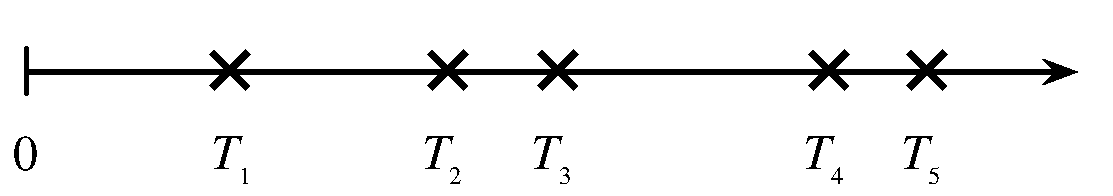
\includegraphics[width=2in]{figures/pp.pdf}
        \end{minipage}}
       
\item[Count-Time Duality]  Consider a Poisson process of emails arriving in an inbox at rate $\lambda$ emails per hour. Let $T_n$ be the time of arrival of the $n$th email (relative to some starting time $0$) and $N_t$ be the number of emails that arrive in $[0,t]$. Let's find the distribution of $T_1$. The event $T_1 > t$, the event that you have to wait more than $t$ hours to get the first email, is the same as the event $N_t = 0$, which is the event that there are no emails in the first $t$ hours. So
\[P(T_1 > t) = P(N_t = 0) = e^{-\lambda t} \longrightarrow P(T_1 \leq t) = 1 - e^{-\lambda t}\]
Thus we have $T_1 \sim \Expo(\lambda)$. By the memoryless property and similar reasoning, the interarrival times between emails are i.i.d.~$\Expo(\lambda)$, i.e., the differences $T_n - T_{n-1}$ are i.i.d.~$\Expo(\lambda)$.
\end{description}

\section{Covariance and Transformations}\hrule height 1pt \smallskip

\subsection{Covariance and Correlation}
\begin{description}
\item [Covariance] is the analog of variance for two random variables.
    \[\cov(X, Y) = E\left((X - E(X))(Y - E(Y))\right) = E(XY) - E(X)E(Y)\]
    Note that 
    \[\cov(X, X) = E(X^2) - (E(X))^2 =  \var(X)\]
\item [Correlation] is a standardized version of covariance that is always between $-1$ and $1$.
    \[\corr(X, Y) = \frac{\cov(X, Y)}{\sqrt{\var(X)\var(Y)}} \]
\item [Covariance and Independence] \hide{If two random variables are independent, then they are uncorrelated. The converse is not necessarily true (e.g., consider $X \sim \N(0,1)$ and $Y=X^2$).}
    \begin{align*}
    	X \independent Y &\longrightarrow \cov(X, Y) = 0 \longrightarrow E(XY) = E(X)E(Y)
    \end{align*}
\item [Covariance and Variance]  The variance of a sum can be found by
    \begin{align*}
        \var(X + Y) &= \var(X) + \var(Y) + 2\cov(X, Y) \\
        \var(X_1 + X_2 + \dots + X_n ) &= \sum_{i = 1}^{n}\var(X_i) + 2\sum_{i < j} \cov(X_i, X_j)
    \end{align*}
    If $X$ and $Y$ are independent then they have covariance $0$, so
    \[X \independent Y \Longrightarrow \var(X + Y) = \var(X) + \var(Y)\]
    If $X_1, X_2, \dots, X_n$ are identically distributed and have the same covariance relationships (often by \textbf{symmetry}), then 
    \[\var(X_1 + X_2 + \dots + X_n ) = n\var(X_1) + 2{n \choose 2}\cov(X_1, X_2)\]
\item [Covariance Properties]  For random variables $W, X, Y, Z$ and constants $a, b$:
    \begin{align*}
    	\cov(X, Y) &= \cov(Y, X) \\
        \cov(X + a, Y + b) &= \cov(X, Y) \\
        \cov(aX, bY) &= ab\cov(X, Y) \\
        \cov(W + X, Y + Z) &= \cov(W, Y) + \cov(W, Z) + \cov(X, Y)\\
        &\quad + \cov(X, Z)
    \end{align*}
\item [Correlation is location-invariant and scale-invariant] For any constants $a,b,c,d$ with $a$ and $c$ nonzero,
    \begin{align*}
        \corr(aX + b, cY + d) &= \corr(X, Y) 
    \end{align*}
\end{description}

\subsection{Order Statistics}
\begin{description}
    \item[Definition] Let's say you have $n$ i.i.d.~r.v.s $X_1, X_2,\dots, X_n$. If you arrange them from smallest to largest, the $i$th element in that list is the $i$th order statistic, denoted $X_{(i)}$. So $X_{(1)}$ is the smallest in the list and $X_{(n)}$ is the largest in the list. \smallskip
    
     Note that the order statistics are \emph{dependent}, e.g., learning $X_{(4)} = 42$ gives us the information that $X_{(1)},X_{(2)},X_{(3)}$ are $\leq 42$ and $X_{(5)},X_{(6)},\dots,X_{(n)}$ are $\geq 42$.
    \item[Distribution]  Taking $n$ i.i.d. random variables $X_1, X_2, \dots, X_n$ with CDF $F(x)$ and PDF $f(x)$, the CDF and PDF of $X_{(i)}$ are:
        \[F_{X_{(i)}}(x) = P (X_{(i)} \leq x) = \sum_{k=i}^n {n \choose k} F(x)^k(1 - F(x))^{n - k}\]
    \[f_{X_{(i)}}(x) = n{n - 1 \choose i - 1}F(x)^{i-1}(1 - F(x))^{n-i}f(x)\]
    \item[Uniform Order Statistics]  The $j$th order statistic of i.i.d.~$U_1,\dots,U_n \sim \Unif(0,1)$ is $U_{(j)} \sim \Beta(j, n - j + 1)$.
\end{description}


\subsection{Conditional Expectation} \smallskip
\begin{description}
    \item[Conditioning on an Event] We can find $E(Y|A)$, the expected value of $Y$ given that event $A$ occurred. A very important case is when $A$ is the event $X=x$. Note that $E(Y|A)$ is a \emph{number}. 
\end{description}
$$E(Y|A) = \int_{-\infty}^\infty yf(y|A)dy$$
\hide{
        \scalebox{0.85}{
                        \setlength{\extrarowheight}{7pt}
            \begin{tabular}{ccc}
                  \textbf{Discrete $Y$} & \textbf{Continuous $Y$} \\
            \toprule
            $E(Y) = \sum_y yP(Y=y)$ & $E(Y) =\int_{-\infty}^\infty yf_Y(y)dy$ \\
            $E(Y|A) = \sum_y yP(Y=y|A)$ & $E(Y|A) = \int_{-\infty}^\infty yf(y|A)dy$ \\ 
            \bottomrule
            \end{tabular}
        }}
\begin{description}
    
    \item[Conditioning on a Random Variable]  We can also find $E(Y|X)$, the expected value of $Y$ given the random variable $X$. \hide{This is \emph{a function of the random variable $X$}. It is \emph{not} a number except in certain special cases such as if $X \independent Y$. To find $E(Y|X)$, find $E(Y|X = x)$ and then plug in $X$ for $x$. For example:
    \begin{itemize}
    \item Let $X \sim \N(0,1)$ and $Y=X^2$. Then $E(Y|X=x) = x^2$ since if we know $X=x$ then we know $Y=x^2$. And $E(X|Y=y) = 0$ since if we know $Y=y$ then we know $X = \pm \sqrt{y}$, with equal probabilities (by symmetry). So $E(Y|X)=X^2, E(X|Y)=0$.  
    \end{itemize} }
    
        \item[Properties of Conditional Expectation] \quad
    \begin{enumerate}
        \item $E(Y|X) = E(Y)$ if $X \independent Y$
        \item $E(h(X)W|X) = h(X)E(W|X)$ (\textbf{taking out what's known}) \\
        In particular, $E(h(X)|X) = h(X)$.
        \item $E(E(Y|X)) = E(Y)$ (\textbf{Adam's Law}, a.k.a.~Law of Total Expectation)
    \end{enumerate}

    \hide{\item[Adam's Law (a.k.a.~Law of Total Expectation)]  can also be written in a way that looks analogous to LOTP. For any events $A_1, A_2, \dots, A_n$ that partition the sample space, 
        \begin{align*}
        E(Y) &= E(Y|A_1)P(A_1) + \dots + E(Y|A_n)P(A_n)
    \end{align*}}
    \item [Adam's Law with Extra Conditioning]
    $$E(E(Y|X, Z)|Z) = E(Y|Z)$$

    \item[Eve's Law (a.k.a.~Law of Total Variance)] \quad
    \[\var(Y) = E(\var(Y|X)) + \var(E(Y|X))\]
\end{description}


\section{MVN, LLN, CLT}\hrule height 1pt \smallskip
\subsection{Sample mean}
Let $X_1, X_2, X_3 \dots$ be i.i.d.~with mean $\mu$. The \textbf{sample mean} is $$\bar{X}_n = \frac{X_1 + X_2 + X_3 + \dots + X_n}{n}$$. Then, $E(\bar{X}_n)=\mu$ and $\var(\bar{X}_n)=\frac{\sigma^2}{n}$.
\subsection{Law of Large Numbers (LLN)}
The \textbf{Law of Large Numbers} states that as $n \to \infty$, $\bar{X}_n \to \mu$ with probability $1$. For example, in flips of a coin with probability $p$ of Heads, let $X_j$ be the indicator of the $j$th flip being Heads.  Then LLN says the proportion of Heads converges to $p$ (with probability $1$).

\subsection{Central Limit Theorem (CLT)}
\subsubsection{Approximation using CLT}
We use $\dot{\,\sim\,}$ to denote \emph{is approximately distributed}. We can use the \textbf{Central Limit Theorem} to approximate the distribution of a random variable $Y=X_1+X_2+\dots+X_n$ that is a sum of $n$ i.i.d. random variables $X_i$. Let  $E(Y) = \mu_Y$ and $\var(Y) = \sigma^2_Y$. The CLT says
\[Y \dot{\,\sim\,} \N(\mu_Y, \sigma^2_Y)\]
If the $X_i$ are i.i.d.~with mean $\mu_X$ and variance $\sigma^2_X$, then $\mu_Y = n \mu_X$ and $\sigma^2_Y = n \sigma^2_X$. For the sample mean $\bar{X}_n$, the CLT says
\[ \bar{X}_n = \frac{1}{n}(X_1 + X_2 + \dots + X_n) \dot{\,\sim\,} \N(\mu_X, \sigma^2_X/n) \]


\subsubsection{Asymptotic Distributions using CLT}

We use $\xrightarrow{D}$ to denote \emph{converges in distribution to} as $n  \to \infty$. \hide{The CLT says that if we standardize the sum $X_1 + \dots + X_n$  then the distribution of the sum converges to $\N(0,1)$ as $n \to \infty$:
\[\frac{1}{\sigma\sqrt{n}} (X_1 + \dots + X_n - n\mu_X) \xrightarrow{D} \N(0, 1)\]
In other words, the CDF of the left-hand side goes to the standard Normal CDF, $\Phi$. In terms of the sample mean, the CLT says}
\[ \frac{\sqrt{n} (\bar{X}_n - \mu_X)}{\sigma_X} \xrightarrow{D} \N(0, 1)\]
\[ \sqrt{n} (\bar{X}_n - \mu_X) \xrightarrow{D} \N(0, \sigma_X^2)\]

\subsection{Markov Chains}\hrule height 1pt \smallskip

\subsubsection{Definition}
\hide{
\begin{minipage}{\linewidth}
            \centering
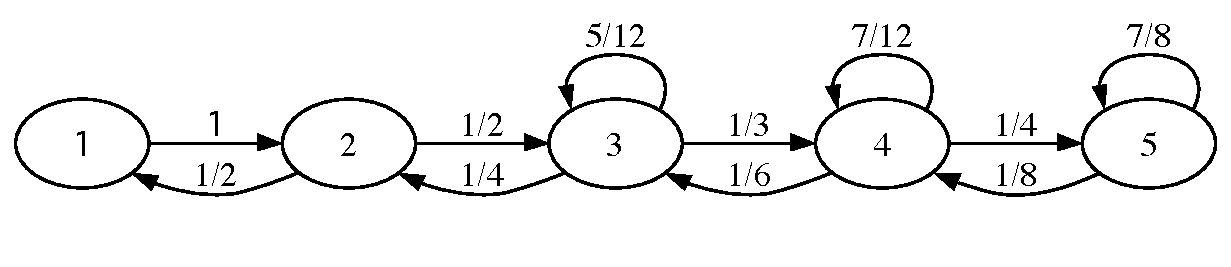
\includegraphics[width=2.3in]{figures/chainA.pdf}
        \end{minipage}
A Markov chain is a random walk in a \textbf{state space}, which we will assume is finite, say $\{1, 2, \dots, M\}$. We let $X_t$ denote which element of the state space the walk is visiting at time $t$. The Markov chain is the sequence of random variables tracking where the walk is at all points in time, $X_0, X_1, X_2, \dots$. By definition, }
A Markov chain must satisfy the \textbf{Markov property}, which says that if you want to predict where the chain will be at a future time, if we know the present state then the entire past history is irrelevant.  \emph{Given the present, the past and future are conditionally independent}. In symbols,
\[P(X_{n+1} = j | X_0 = i_0, X_1 = i_1, \dots, X_n = i) = P(X_{n+1} = j | X_n = i)\]
\hide{
\subsubsection{State Properties}
A state is either recurrent or transient.
\begin{itemize}
\item If you start at a \textbf{recurrent state}, then you will always return back to that state at some point in the future.  \textmusicalnote \emph{You can check-out any time you like, but you can never leave.}  \textmusicalnote
\item Otherwise you are at a \textbf{transient state}. There is some positive probability that once you leave you will never return. \textmusicalnote \emph{You don't have to go home, but you can't stay here.} \textmusicalnote
\end{itemize}
A state is either periodic or aperiodic.
\begin{itemize}
\item If you start at a \textbf{periodic state} of period $k$, then the GCD of  the possible numbers of steps it would take to return back is  $k>1$.
\item Otherwise you are at an \textbf{aperiodic state}. The GCD of  the possible numbers of steps it would take to return back is 1.
\end{itemize}
\textbf{Number of returns to transient state is Geometric:} Suppose the probability of never returning to
$i$, starting from $i$, is a positive number $p > 0$. Then, starting from $i$, the number of
times that the chain returns to $i$ before leaving forever is distributed $\Geom(p)$.}


\subsubsection{Transition Matrix}
Let the state space be $\{1,2,\dots,M\}$. The transition matrix $Q$ is the $M \times M$ matrix where element $q_{ij}$ is the probability that the chain goes from state $i$ to state $j$ in one step:
\[q_{ij} = P(X_{n+1} = j | X_n = i)\]

To find the probability that the chain goes from state $i$ to state $j$ in exactly $m$ steps, take the $(i, j)$ element of $Q^m$.
\[q^{(m)}_{ij} = P(X_{n+m} = j | X_n = i)\]
If $X_0$ is distributed according to the row vector PMF $\vec{p}$, i.e., $p_j = P(X_0 = j)$, then the PMF of $X_n$ is $\vec{p}Q^n$. The number of free parameters in this system depends on how many free parameters are in the transition matrix.



\subsubsection{Chain Properties}
A chain is \textbf{irreducible} if you can get from anywhere to anywhere. If a chain (on a finite state space) is irreducible, then all of its states are recurrent. A chain is \textbf{periodic} if any of its states are periodic, and is \textbf{aperiodic} if none of its states are periodic. In an irreducible chain, all states have the same period. \smallskip

A chain is \textbf{reversible} with respect to $\vec{s}$ if $s_iq_{ij} = s_jq_{ji}$ for all $i, j$.  Examples of reversible chains include any chain with $q_{ij} = q_{ji}$, with $\vec{s} = (\frac{1}{M}, \frac{1}{M}, \dots, \frac{1}{M})$, and random walk on an undirected network.

\subsubsection{Stationary Distribution}

Let us say that the vector $\vec{s} = (s_1, s_2, \dots, s_M)$ be a PMF  (written as a row vector). We will call $\vec{s}$ the \textbf{stationary distribution} for the chain if $\vec{s}Q = \vec{s}$. \hide{As a consequence, if $X_t$ has the stationary distribution, then all future $X_{t+1}, X_{t + 2}, \dots$ also have the stationary distribution.} 

For irreducible, aperiodic chains, the stationary distribution exists, is unique, and $s_i$ is the long-run probability of a chain being at state $i$. The expected number of steps to return to $i$ starting from $i$ is $1/s_i$.

\smallskip

 To find the stationary distribution, you can solve the matrix equation $(Q' - I){\vec{s}\,}'= 0$. The stationary distribution is uniform if the columns of $Q$ sum to 1. This is true for symmetric matrices

\smallskip

\textbf{Reversibility Condition Implies Stationarity}  If you have a PMF $\vec{s}$ and a Markov chain with transition matrix $Q$, then $s_iq_{ij} = s_jq_{ji}$ for all states $i, j$ implies that $\vec{s}$ is stationary. 

\textbf{Columns Summing to One Implies Stationarity} If each column of the transition matrix $Q$ sums to 1, then the uniform distribution over all the states, $(1/M,1/M,\dots,1/M)$ is a stationary distribution. One example of this is a \underline{symmetric transition matrix}\hide{ (in which case it's also reversible)}.

\subsubsection{Random Walk on an Undirected Network}
 \hide{\begin{minipage}{\linewidth}
            \centering
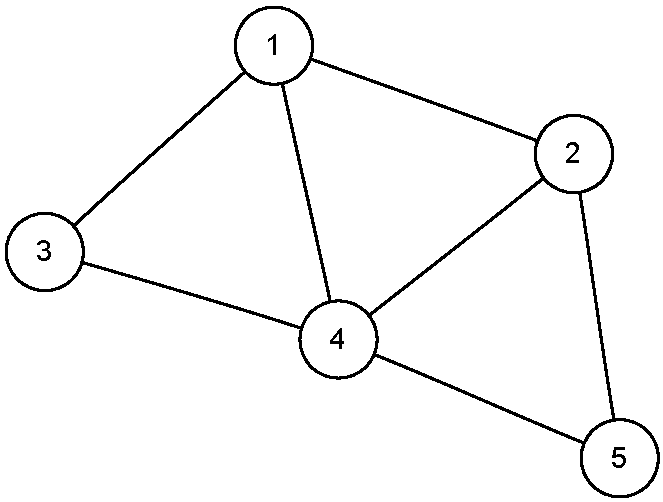
\includegraphics[width=0.2\columnwidth]{figures/network1.pdf}
        \end{minipage}}


\hide{If you have a collection of \textbf{nodes}, pairs of which can be connected by undirected \textbf{edges}, and a Markov chain is run by going from the current node to a uniformly random node that is connected to it by an edge, then  this is a random walk on an undirected network. }The stationary distribution of a random walk chain is proportional to the \textbf{degree sequence} (this is the sequence of degrees, where the degree of a node is how many edges are attached to it). For example, the stationary distribution of random walk on the network shown above is proportional to $(3,3,2,4,2)$, so it's $(\frac{3}{14}, \frac{3}{14}, \frac{3}{14}, \frac{4}{14}, \frac{2}{14})$. 

\hide{
\subsection{Metropolis Algorithm}
Let $\vec{s}$ be the desired stationary distribution. Let $P$ be a transition matrix for some chain on the space. From state $i$:
\begin{enumerate}
\item Generate a proposal state $j$, according to $P$.
\item Accept or reject proposal with $a_{ij}=\min(\frac{s_jp_{ji}}{s_i p_{ij}}, 1)$
\end{enumerate}
This gives transition matrix $Q$ with $q_{ij}=p_{ij}a_{ij}$ if $i\neq j$, and $q_{ii}=p_ii+\sum_{j\neq 1} p_{ij} (1-q_{ij})$ if $i=j$. We can show this is reversible.
}

\section{Inequalities} \hrule height 1pt \smallskip

\begin{enumerate}
\itemsep0em
\item \textbf{Cauchy-Schwarz} $|E(XY)| \leq \sqrt{E(X^2)E(Y^2)}$
\item \textbf{Markov} $P(X \geq a) \leq \frac{E|X|}{a}$ for $a>0$
\item \textbf{Chebyshev} $P(|X - \mu| \geq a) \leq \frac{\sigma^2}{a^2}$ for $E(X)=\mu, \var(X) = \sigma^2$. Useful for proving convergence in probability; to prove consistency of estimator we just need to show that its variance goes to 0.
\item \textbf{Jensen} $E(g(X)) \geq g(E(X))$ for $g$ convex; reverse if $g$ is concave
\item \textbf{Chernoff's} For any r.v. $X$ with finite mean $\mu$ and constant $a,t > 0$, $P(X \geq a) \leq \frac{E(e^tX)}{e^{ta}}$
\end{enumerate}


\section{Formulas} \hrule height 1pt \smallskip
\begin{enumerate}
    \itemsep0em
    \item \textbf{Geometric Series } \\
    $1 + r + r^2 + \dots + r^{n-1} = \sum_{k=0}^{n-1} r^k = \frac{1 - r^n}{1 -r}$
    $1 + r + r^2 + \dots = \frac{1}{1-r} \textnormal{ if $|r|<1$}$
    \item $\mathbf{e^x} = \sum_{n=0}^\infty \frac{x^n}{n!}= 1 + x + \frac{x^2}{2!} + \frac{x^3}{3!} + \dots = \lim_{n \rightarrow \infty} \left( 1 + \frac{x}{n} \right)^n$
    \item \textbf{Binomial Theorem} $(x+y)^n=\sum_{k=0}^n {n\choose k} x^k y^{n-k}=\sum_{k=0}^n {n\choose k} x^{n-k} y^k$
    \item \textbf{Gamma and Beta Integrals}
    $ \int_0^\infty x^{t-1}e^{-x}\, dx = \Gamma(t) \hspace{1 cm} \int_0^1 x^{a - 1}(1-x)^{b-1}\, dx = \frac{\Gamma(a)\Gamma(b)}{\Gamma(a + b)}$
    Also, $\Gamma(a+1) = a \Gamma(a)$, and $\Gamma(n) = (n - 1)!$ if $n$ is a positive integer. 
    \item $\sum_n (X_j - \bar X)(Y_j - \bar Y) = \sum_n X_jY_j - n\bar X \bar Y$
    \item $nE(\bar X \bar Y) = \frac{1}{n}\sum_{i,j}E(X_iY_i) = \frac{1}{n}(nE(X_1Y_1) + n(n-1)E(X_1Y_2))$
\end{enumerate}

\section{STAT 111 Stuff} \hrule height 1pt
\subsection{Summary Statistics}
\begin{description}
\item[Medians and Quantiles] Let $X$ have CDF $F$. Then $X$ has median $m$ if $F(m) \geq 0.5$ and $P(X \geq m) \geq 0.5$. For $X$ continuous, $m$ satisfies $F(m)=1/2$. In general, the $a$th quantile of $X$ is $\min \{x: F(x)\geq a\}$; the median is the case $a=1/2$.
\item[Standard Error] $SE(\hat \theta) = \sqrt{\var(\hat \theta)}$
\end{description}

\subsection{Likelihood}
\hide{Let $f_{\vec Y}$ be a model for the joint density function of all the observations. Let $\vec{y}$ be the observed value of $\vec{Y}$. Then the likelihood function is:}
\[ L(\theta;\vec y)=f_{\vec{Y}}(y|\theta) \]
It is regarded as a function of $\theta$, with $y$ treated as fixed.
\begin{description}
\item[Frequentist Interpretation] $\theta$ is regarded as fixed but unknown, and it does not have a distribution. \hide{If $L(\theta_2)>L(\theta_1)$, strictly speaking we cannot say that $\theta_2$ is more likely than $\theta_1$ to be the true value of $\theta$. However, we can say that $\theta$ seems more plausible than $\theta$ as a source for generating the data.}
\item[Bayesian Interpretation]
We have a prior density $g(\theta)$ for $\theta$, then:
\[L(\theta)=g(\theta|\vec{y}=\frac{g(\theta)f(y|\theta)}{f(\vec{y})}\propto g(\theta)f(y|\theta)=L(\theta)g(\theta)\]
So the posterior is proportional to likelihood times prior.
\item[Equivalence] Two likelihood functions are viewed as equivalent if one is a positive constant times the other. In fact, the ``constant'' can even be function of the data (it just can’t depend on the parameter).
\item[Invariance] Let $\psi=g(\theta)$ be a reparametrization, where $g$ is a one-to-one function. Then $L(\psi;\vec{y}=L(\theta;\vec{y})$.
\end{description}
\subsection{Estimands, Estimators, \& Estimates}
\begin{description}
\hide{
\item[Statistic] A statistic is a function of $Y_1,...,Y_n$ (and possibly other known quantities). We can write a statistic as $T(Y)$, where computing the function $T$ must not require knowing any unknown parameters. \underline{Note:} The \textit{distribution} of a statistic can depend on unknown parameters.}
\item[Estimand] An estimand is an object that we wish to learn about from data.
\item[Estimator] An estimator $\hat\theta=T(\vec{Y})$ is a statistic with the intention of estimating an estimand $\theta$.
\item[Estimate] An estimate is a realization of an estimator. If $T(Y)$ is an estimator of some estimand $\theta$, then $T(y)$ is an estimate of $\theta$.
\end{description}
\subsection{Method of Moments}
Set the expectation of the sample moments equal to the actual sample moments. Compute the expectation in terms of the unknown parameter(s) and rearrange to get the estimator. Write as many equations as you have parameters, one equation per moment. For example, suppose you have unknown parameters $\theta$ and $\lambda$.
\begin{align*}
    \text{1st moment } E(\frac{1}{n}\sum X_i) = f(\theta, \lambda) \\
    \text{2nd moment } E(\frac{1}{n}\sum X_i^2) = f(\theta, \lambda) \\
\end{align*}
You can then solve this system of equations for $\hat \theta$ and $\hat lambda$. 
\subsection{Maximum Likelihood Estimation}
The \textbf{maximum likelihood estimate} of $\theta$ is the value $\hat\theta$ that maximizes the likelihood function $L(\theta; y)$. \hide{The corresponding estimator is called the \textbf{maximum likelihood estimator}. That is, if the maximum likelihood estimate is $T(y)$, then the maximum likelihood estimator is $T(Y)$.}
\begin{description}
\item[Regularity conditions] Support must not depend on the value of the estimand. The estimate $\theta^*$ must not be on the boundary. You must be able to Differentiate under the Integral Sign, i.e. $\frac{d}{d\theta} \int g(y)f_\theta(y)dy = \int \frac{d}{d\theta} g(y)f_\theta(y)dy$. The estimand must be of a fixed dimension.
\item[Invariance] If $\hat\theta$ is the MLE of $\theta$, then $g(\hat\theta)$ is the MLE of $\hat\theta$.
\item[Consistency] The MLE $\hat\theta$ is consistent, which means that it converges in probability to the true $\theta$.
\item[Asymptotically Normal] The MLE is asymptotically Normal (so its distribution is approximately Normal if the sample size is large).
\item[Asymptotically unbiased] The MLE is asymptotically unbiased (the bias approaches 0 as the sample size grows).
\item[Asymptotically efficient] The MLE is asymptotically efficient (no other asymptotically unbiased estimator will have a lower standard error asymptotically).
\end{description}
\subsection{Bias, Variance and Loss Functions}
\begin{description}
\item[Bias] The bias of an estimator $\hat\theta$ for $\theta$ is $E(\hat\theta)-\theta$.
\item[Loss function] A loss function is a function $L(\theta,\hat\theta)$, interpreted as the loss associated with using the estimate $\hat\theta$ when the true parameter value is $\theta$. We require that $L(\hat\theta,\theta)\geq 0$ and $L(\theta,\theta)=0$.
\item[Mean squared error] The mean squared error is $E(\hat\theta-\theta)^2$.
\item[Bias-variance decomposition] We know $\MSE_{\theta}=\var_\theta(\hat\theta)+(\bias_\theta(\hat\theta))^2$. This illustrates the \textit{bias-variance tradeoff}.
\end{description}
\hide{\section{Estimators for CDF and PDF}}
\subsection{Kernel Density Estimation}
Suppose the estimand is the density of $Y_1$ at a particular point $y_1$: $\theta=f_{Y_1}(y_1)$. The kernel density estimator is:
\[\hat f_n(y)=\frac{1}{n}\frac{1}{h}K(\frac{Y_i-y}{h})\]
where $h>0$ is called the \textit{bandwidth} and $K$ is called the \textit{kernel function}. The kernel function must be a PDF (nonnegative and summing to 1). For instance, the Gaussian kernel takes $K$ to be a Normal PDF centered at 0. \hide{The intuitive idea of the KDE for the Gaussian case is to place a little Normal distribution centered at each data point, and then mix all these Normal distributions together to obtain a single smooth PDF. The bandwidth
$h$ controls how tightly concentrated or spread out each of the $n$ little Normal PDFs
is about the $y$ it is centered at.}
\section{Asymptotics and Information} \hrule height 1pt
\subsection{Consistency}
An estimator $\hat\theta$ is \textbf{consistent} for the estimand $\theta$ if $\hat\theta$ converges in probability to the true $\theta$ as the sample size $n\to\infty$, i.e. for every $\epsilon>0$, we have $\lim_{n\to\infty} P(|\hat\theta-\theta|\geq\epsilon)=0$.

\begin{description}
\item[Sufficient condition] If $\MSE(\hat\theta)\to 0$ as $n\to\infty$, then $\hat\theta$ is consistent. In particular, if $\bias(\hat\theta)\to 0$ and $\var(\hat\theta)\to 0$ as $n\to\infty$, then $\hat\theta$ is consistent.
\end{description}
\subsection{Kullback-Leibler Divergence}
The \textbf{Kullback-Leibler  divergence} is a way to compare two distributions; it measures the impact on expected log-likelihood if we use an approximate distribution as a proxy for the true distribution. It is defined to be:
\[K(\theta^*,\theta)=E\left(\log\frac{L(\theta^*;\vec{Y)}}{L(\theta;\vec Y)}\right)=E(\log(L(\theta^*;\vec{Y})-E(\log(L(\theta;\vec{Y})\]
where the expectation is computed under the distribution $\vec{Y}\sim F_\vec{Y}(\vec{y}|\theta^*)$.

\begin{description}
\item[Nonnegative] For any $\theta$, we have $K(\theta^*,\theta)\geq 0$. The inequality is strict unless $F_\vec{Y}(\vec{y}|\theta^*)$ and $F_\vec{Y}(\vec{y}|\theta)$ are the same distribution. In particular, $\theta^*$ maximizes the expected log-likelihood. the MLE $\hat\theta$ is where the \textit{observed} log-likelihood function has its peak, while $\theta^*$ is where the \textit{expected} log-likelihood function has its peak, thus lending support for using MLEs. Note that graders may require you to check the second derivative $l''(\theta) < 0$ to confirm you have found a maximum and not a minimum.
\end{description}
\subsection{Score function and Fisher information}
\begin{description}
\item[Score function]
The score function is $s=\frac{\partial l(\theta;y)}{\partial\theta}$.

\hide{
As defined, the score function depends on both $\theta$ and on $\vec y$. In some applications, such as when finding the MLE, we fix $y$ and look at $s(\theta;y)$ as a function of $\theta$.  

In other applications,it turns out to be useful to fix $\theta$ at its true value $\theta^*$ and look at the random variables $(\theta^*;Y)$. In still other applications, we are interested in some specific hypothesized parameter $\theta_0$and we look at the statistics $(\theta_0;Y)$ (note that $s(\theta^*;Y)$ is \textit{not} a statistic since $\theta^*$ is unknown).}

We have that:
\begin{align*}
E(s(\theta^*;\vec Y))&=0 \\
\var(s(\theta^*;\vec Y)&=-E(s'(\theta^*;\vec Y))
\end{align*}
\item[Fisher information]
The Fisher information for a parameter $\theta$ is:
\[I(\theta)=\var_\theta s(\theta;\vec Y)\]
where the subscript of $\theta$ indicates that we compute the variance under the assumption that the  true  parameter  value is $\theta$. We  will  sometimes  write $I_n(\theta)$  for  the  Fisher information when the sample size is $n$.

\item[Fisher information of function of r.v.] Let $\tau=g(\theta)$, where $g$ is a differentiable function with $g'(\theta)\neq 0$. Then:
\[I(\tau)=\frac{I(\theta)}{(g'(\theta))^2}\]
\end{description}

\subsection{Cramer-Rao Lower Bound}
Let $\hat \theta$ be an unbiased estimator of $\theta$. Under regularity conditions, $$Var(\hat \theta) \geq \frac{1}{\I(\theta^*)}$$. Since bias is 0, variance = MSE of the estimator. 
For $\theta$ which may be biased, this becomes $$Var(\hat \theta) \geq \frac{g'(\theta^*))^2}{\I(\theta^*)}$$ where $E(\hat \theta) = g(\theta^*)$.

\subsection{Asymptotic distribution of the MLE}
For large sample size, it is \textit{approximately} true that the MLE is Normal, unbiased, and achieves the CRLB.

Under regularity conditions, the asymptotic distribution of $\hat\theta$ is given by:
\[\sqrt n (\hat\theta-\theta^*)\todist \N\left(0, \frac{1}{I_1(\theta^*)}\right)\]
as the sample size $n\to\infty$. As an \textit{approximation}, the result says that for large $n$,
\[\hat\theta\asim \N\left(\theta^*,\frac{1}{nI_1(\theta^*)}\right)\]
\subsection{Delta Method}
The \textit{delta method} says that if:
\[\sqrt{n}(\hat{\theta} - \mu)\todist \N(0,\sigma^2)\] and $g$ is a differentiable function, then: \[\sqrt{n}(g(\hat{\theta}) - g(\mu))\todist \N(0, (g'(\mu))^2 \sigma^2)\]
\subsection{Interval Estimation}
Use a pivot to write a function of the estimator of interest that has a distribution whose parameters are known (ex. changing $X \sim \Expo(\lambda)$ to $\lambda X \sim \Expo(1)$. This known distribution also has a known CDF whose function you can use to construct the confidence interval.
\subsection{Sufficient Statistics}
\subsubsection{Definition of Sufficient Statistics}
Let $\textbf{Y} = (Y_1,..Y_n)$ be a sample from model $F_y(y|\theta)$. A statistic $T(Y)$ is a sufficient statistic for $\theta$ if conditional distribution of $Y|T$ does not depend on $\theta$.
\subsubsection{Factorization Criterion}
T(Y) is a sufficient statistic if and only if we can factor $$f_y(y|\theta) = g(T(y),\theta)h(y)$$ where $f_y(y|\theta)$ is the PMF/PDF of $Y$.
\subsubsection{Rao-Blackwell}
Let T be a sufficient statistic and $\hat \theta$ be any estimator for $\theta$. Then the MSE of the Rao-Blackwellized estimator $\hat \theta_RB = E(\theta |T)$ does not exceed the MSE of the original estimator. This can be proven with the bias-variance decomposition and Adam and Eve's Laws.
\subsection{Natural Exponential Family}
 An r.v. follows NEF if its PDF is in the form $$f_y(y|\theta) = e^{\theta y - \Psi(\theta)}h(y)$$ Where $\theta$ is the natural parameter. Note that $\theta$ doesn't necessarily have to be a parameter of interest, e.g. it could be $-\mu$ instead of $\mu$ for a normal distribution.
\subsubsection{Properties}
If $Y$ is in NEF form (e.g. Normal ($\sigma^2$ known), Poisson, Binomial (n fixed), Negative Binomial (r fixed), $\Gamma(a, \lambda)$ (a known), then we have the following facts.
\begin{enumerate}
    \item $E(Y) = \Psi'(\theta), \var(\theta) = \Psi''(\theta)$, MGF $M_y(t) = E(e^{tY}) = e^{\Psi(\theta + t) - \Psi(\theta)}$.
    \item $\bar Y$ is a sufficient statistic for $\theta$.
    \item MLE for mean paramter $\mu = E(Y)$ is $\mu = \bar Y$.
    \item Fisher Information $I_1(\theta) = \Psi''(\theta)$.
\end{enumerate}

\subsection{MLEs \& Fisher Informations}
\begin{itemize}
    \itemsep0em
    \item Bernoulli: $\hat p = \bar Y$. $I_1(p) = \frac{1}{pq}$
    \item Binomial: $\hat p = \frac{y}{n}$. $I_n(p) = \frac{n}{pq}$
    \item Geometric: $\hat p = n/\sum y_i$. $I_n(p) = n(\frac{1}{p^2} + \frac{1}{pq})$
    \item Negative binomial: $\hat p = \frac{r}{\bar Y + r}$. $I_1(p) = \frac{r}{q^2p}$
    \item Poisson: $\hat \lambda = \frac{1}{n}\sum y_i$. 
    $I_1(\lambda) = \frac{1}{\lambda}$
    \item Exponential: $\hat \lambda = n/\sum y_i = 1 / \bar Y$. $I_1(\lambda) = \lambda^{-2}$
    \item Normal: $\hat \mu = \bar Y$. $\hat \sigma^2 = \frac{1}{n} \sum (y_i - \bar Y)^2$
    \item Weibull: $\hat \lambda|\gamma = \frac{1}{n}\sum y_i^\gamma$
\end{itemize}

\subsection{Student-t Distribution}
Let $T = \frac{E}{\sqrt{V/n}}$ where $Z \sim \N(0, 1)$ and $V \sim \chi_n^2$ (remember, special case of Gamma) where $Z \independent V$, then $T \sim \stu_n$ (where $n$ is called the \# of degrees of freedom). If $n = 1$, then $T \sim \textnormal{Cauchy}$. Can find mean, variance, in your head by remembering it's a sum of standard Normals.

\textbf{Also:} For $Z_1,\dots,Z_n\simiid \N(0,1)$, we can find using JFI that $\sum_{j=1}^n (Z_j-\bar{Z_n})^2\sim \chi^2_{n-1}$.

\section{Linear Regression} \hrule height 1pt
\begin{description}
\item[Regression function] $r(x) = E(Y| X = x) = \int yf(y|x) \, dy$. \\  Assume data is $\{(Y_1, X_1), \dots, (Y_n, X_n)\}, \text{ i.i.d. }F_{Y, X}$

\item[Simple Linear Regression Model] $Y_i = \beta_0 + \beta_1 X_i + \epsilon_i$ \\
where $E(\epsilon_i | X_i = x) = 0$ and $\var(\epsilon_i | X_i = x) = \sigma^2$ \\
Predicted or fitted values: $\hat{Y_i} = \hat\beta_0 + \hat\beta_1 x$

\item[Residual Sums of Squares] $\sum_{i = 1}^n \hat\epsilon_i^2$ 

\item[Least Squares Estimators] MLEs are assuming that errors are normally distributed
\begin{align*}
    \hat\beta_1 &= \frac{\sum_{i = 1}^n (Y_i - \bar{Y})(X_i - \bar{X})}{\sum_{i = 1}^n (X_i - \bar{X})^2} \text{ (MLE)}\\
    \hat\beta_0 &= \bar{Y} - \hat\beta_1\bar{X} \text{ (MLE)}\\
    \hat\sigma^2 &= \frac{1}{n - 2} \sum_{i = 1}^n \hat\epsilon_i^2 \text{(unbiased, not MLE)}
\end{align*} 

\item[Asymptotic Distribution] $\sqrt{n}(\hat\beta_1 - \beta_1) \stackrel{d}{\to} \N\left(0, \frac{\sigma^2}{\sigma^2_X}\right)$

\item[Student-t Distribution] Let $\hat\sigma^2$ as above, and let $s_{xx}^2 = \sum_{i = 1}^n (x_i - \bar{x})^2$. Then
\begin{align*}
    \frac{\hat\beta_1 - \beta_1}{\hat\sigma/s_{xx}} \sim t_{n - 2}
\end{align*} 

\item[Prediction] We see a new $X = x_0$ and want to predict new $Y$. Predict $Y$ with estimators, $\hat{Y} = \hat\beta_0 + \hat\beta_1 x_0$.
\begin{align*}
    E(\hat{Y} - Y | \vec{X} = \vec{x}) &= 0 \\ 
    \var(\hat{Y} - Y | \vec{X} = \vec{x}) &= \sigma^2 \left(\frac{1}{n} + \frac{(x_0 - \bar{x})^2}{s_xx^2} + 1 \right) \\ 
    \frac{\hat{Y} - Y}{\hat\sigma \sqrt{\frac{1}{n} + \frac{(x_0 - \bar{x})^2}{s_xx^2} + 1}} &\sim t_{n - 2}
\end{align*} 
The $1 - \alpha$ confidence interval for $Y$ is
\begin{align*}
    \hat{Y} \pm t^{-1}_{n - 2}(\alpha / 2) \hat\sigma \sqrt{\frac{1}{n} + \frac{(x_0 - \bar{x})^2}{s_xx^2} + 1}
\end{align*}
\end{description}

\subsection{Slutsky's and Continuous Mapping Theorem}
\begin{description}
\item[Slustky's Theorem] If $X_1, X_2 \dots$ and $Y_1, Y_2, \dots$ are sequences of random variables such that $X_n \stackrel{d}{\to} X$ and $Y_n \stackrel{p}{\to} c$, then
\begin{enumerate}
\itemsep0em
\item $X_n + Y_n \stackrel{d}{\to} X + c$
\item $X_n Y_n \stackrel{d}{\to} cX$ 
\item if $c \neq 0$, then $X_n/Y-n \stackrel{d}{\to} X/c$
\end{enumerate} 
\item[Continuous Mapping Theorem] If $X_1, X_2, \dots$ are sequences of random variables and $g$ is a continuous function, then
\begin{enumerate}
\itemsep0em
\item if $X_n \stackrel{d}{\to} X$, then $g(X_n) \stackrel{d}{\to} g(X)$.
\item if $X_n \stackrel{p}{\to} c$, then $g(X_n) \stackrel{p}{\to} g(c)$.
\end{enumerate}


\end{description}

\section{Hypothesis Testing} \hrule height 1pt
\subsection{Null and Alternative Hypotheses}
\begin{description}
\item[Hypothesis Testing Framework] Partition parameter space $\Theta$ into two disjoint sets, $\Theta = \Theta_0 \cup \Theta_1$
\item[Null Hypothesis] $H_0 : \theta \in \Theta_0$. Simple if it consists of a single point. Composite if not simple. 
\item[Alternative Hypothesis] $H_1 : \theta \in \Theta_1$.
\item[Rejection Region] Set $R$ of possible values $\vec{y}$ for the data such that we reject the null hypothesis $\vec{y} \in R$. Usually of the form $R = \{\vec{y} : t(\vec{y}) > c\}$ or $R = \{\vec{y} : t(\vec{y}) > c_U \text{ or } t(\vec{y}) < c_L\}$. Often, $c$ is some quantile, $F^{-1}(\alpha)$.
\item[Type I Error] $\theta \in \Theta_0$ but $\vec{y} \in R$ (incorrectly reject null).
\item[Type II Error] $\theta \in \Theta_1$ but $\vec{y} \notin R$ (incorrectly fail to reject).
\item[One-sided test] $H_0 : \theta = \theta_0$ vs $H_1: \theta \neq \theta_0$
\item[Two-sided test] $H_0 : \theta \leq \theta_0$ vs $H_1 : \theta > \theta_0$.    
\end{description}

\subsection{Size and Power}
\begin{description}
\item[Power function] $\beta(\theta) = P(\vec{Y} \in R|\theta)$. How likely we are to reject for a given true parameter value. Typically, power of a test refers to $\beta(\theta)$ for $\theta \in \Theta_1$.
\item[Size] Size or level of a test is the maximum possible Type I error probability. $\alpha = \max_{\theta \in \Theta_0} \beta(\theta)$.
\end{description}

\subsection{z-test}
\reminder

\subsection{t-test}
Let 
\begin{align*}
    \hat\sigma^2 &= \frac{1}{n - 1}\sum_{i = 1}^n (Y_i - \bar{Y})^2 \\
    T(\vec{Y}) &= \frac{\bar{Y} - \mu_0}{\hat\sigma / \sqrt{n}} \\
    \implies T(\vec{Y}) &\sim t_{n - 1}
\end{align*}

\subsection{p-values}
A \textbf{p-value} is the smallest $\alpha$ (Type I error rate) at which we could have rejected $H_0$, so
\begin{align*}
    p = \inf{\alpha : y \in R_\alpha}
\end{align*}
Often, our rejection region is of the form $R = \{\vec{y} : T(\vec{y}) > F^{-1}(\alpha)\}$. In this case, we can calculate $p = F(t(\vec{y}))$. \\ 
\textbf{Theorem: } Let $T$ be a continuous test statistic, and suppose we are using a hypothesis test that rejects $H_0 : \theta = \theta_0$ when $T$ is large. As a random variable, the p-value is $\Unif(0, 1)$ under $H_0$. 

\subsection{Misc Tests}
\begin{description}
\item[Wald Test] Under some regularity conditions, $\hat\theta \stackrel{\cdot}{\sim} \N(\theta_0, I^{-1}(\theta_0))$. So, can use the test statistic,
\begin{align*}
    t(\vec{Y}) = \sqrt{I(\theta_0)}(\hat\theta - \theta_0) \sim \N(0, 1)
\end{align*} 
\item[Score test] Under some regularity conditions, $s(\vec{y}, \theta_0)$ is asymptotically Normal.
\begin{align*}
    \frac{s(\vec{y}; \theta_0)}{\sqrt{\I(\theta_0)}} \sim \N(0, 1)
\end{align*} 
\item[Likelihood Ratio Test (LRT)] If testing a simple null vs simple alternative, then Neyman-Pearson lemma says most powerful test will be based on likelihood ratio 
\begin{align*}
    LR = \frac{L(\theta_1, \vec{Y})}{L(\theta_0, \vec{Y})}
\end{align*} 
The more general LRT is given by
\begin{align*}
    LR = \frac{L(\hat\theta; \vec{Y})}{L(\theta_0; \vec{Y})}
\end{align*}
We also have the folllowing theorem under some mild regularity theorems, 
\begin{align*}
    \Lambda(\vec{Y}) &= 2 \log\left(\frac{L(\hat\theta, \vec{Y})}{L(\theta_0; \vec{Y})}\right) \stackrel{D}{\to} \chi_1^2
\end{align*}
\end{description}

\section{Causal Inference} \hrule height 1pt
\begin{description} 
\item[Potential Outcomes] Treat $X \in \{0, 1\}$ is treatment assignment. We observe potential outcomes
\begin{align*}
    Y = \begin{cases}
        Y(1) & \text{if } X = 1 \\ 
        Y(0) & \text{if } X = 0
    \end{cases}
\end{align*}
\item[Average Causal Effect] $\theta = E[Y(1) - Y(0)]$
\item[Association] $\alpha = E[Y(1) \mid X = 1] - E[Y(0) \mid X = 0]$

In general, $\alpha \neq \theta$
\item[Unbiased Estimator] $ \hat\theta = \bar{Y_1} - \bar{Y_0} = \hat\beta_1$
\end{description}   

\section{Sampling} \hrule height 1pt
\subsection{Simple Random Sampling (SRS)}
\begin{description}
\item[Definition] An SRS of size $n$ from a population of size $N$ is a random sample of size $n$, chosen without replacement, such that all possible samples are equally likely. $Y_j$ is $j$th individual sampled, $y_i$ is person with label $i$ in population.     
\item[Sample Mean] Sample mean is unbiased
\begin{align*}
    E(\bar{Y}) &= \mu \\
    \var(\bar{Y}) &= \frac{\sigma^2}{n} \cdot \frac{N - n}{N - 1} \\
\end{align*} 
\item[Covariance] 
\begin{align*}
    \cov(Y_i, Y_j) &= \frac{-\sigma^2}{N - 1}
\end{align*} 
\end{description}
\subsection{Stratified Random Sampling}
\begin{description}
\item[Definition] Suppose that the population is partitioned into $L$ subpopulations called \textit{strata}. Let $N_\ell$ be the size of stratum $\ell$, so $N_1 + \dots + N_L = N$. Assume $N_\ell \geq 2 \forall \ell$. Within each stratum $\ell$, an SRS of size $n_\ell$ is drawn, for soome predetermined $n_\ell$. Let $y_{i, \ell}$ be the $y$ values within the stratum $\ell$, let $\mu_\ell$ be the population mean within stratum $\ell$ and let $\sigma_\ell^2$ be the population variance in stratum $\ell$, 
\begin{align*}
    \mu_\ell = \frac{1}{N_\ell} \sum_{i = 1}^{N_\ell} y_{i, \ell} \text{ and } \sigma_\ell^2 = \frac{1}{N_\ell}\sum_{i = 1}^{N_\ell} (y_{i, \ell} - \mu_\ell)^2
\end{align*} 
\item[Estimator] The stratified sampling estimator $\bar{Y}_{\text{strat}}$ is
\begin{align*}
    \bar{Y}_{\text{strat}} = \sum_{\ell = 1}^L \frac{N_\ell}{N} \cdot \bar{Y}_\ell
\end{align*}
This estimator is unbiased. The variance is:
\begin{align*}
    \var\left(\bar{Y}_{\text{strat}}\right) = \sum_{\ell = 1}^L \left(\frac{N_\ell}{N}\right)^2 \cdot \frac{\sigma_\ell^2}{n_\ell} \cdot \frac{N_\ell - n_\ell}{N_\ell - 1}
\end{align*}
\item[Optimal Allocation] In terms of minimizing MSE, the optimal allocation of sampling is
\begin{align*}
    n_\ell &= \frac{n N_\ell \tilde\sigma_\ell}{\sum_{k = 1}^L N_k \tilde\sigma_k} \\
    \implies n_\ell &\propto N_\ell \tilde\sigma_\ell
\end{align*} 
Where $\tilde\sigma_\ell$ is the standard deviation in stratum $\ell$ except defined with $N_\ell - 1$ in the denominator rather than $N_\ell$. 
If there is a cost per sample $c_\ell$ in each stratum and a total budget, then $n_\ell \propto \frac{N_\ell \tilde\sigma_\ell}{\sqrt{c_\ell}}$. 
\end{description}

\subsection{Horvitz-Thompson Estimator}
Let $S$ be the set of distinct ID numbers members of a random sample from the population. Let $\pi_i = P(i \in S)$ be the probability that individual $i$ is included in the sample. Assume that $\pi_i$ are known in advance and that $\pi_i > 0 \forall i$, then the \textit{Horvitz-Thomspon} estimator
\begin{align*}
    \tau_{\text{HT}} \sum_{i \in S} \frac{y_i}{\pi_i}
\end{align*}
is \textbf{unbiased} for the population total $\tau = y_1 + \dots + y_N$.\\ 
If $N$ is known, then 
\begin{align*}
    \hat\mu_{\text{HT}} = \frac{\hat\tau_{\text{HT}}}{N}
\end{align*}
is an unbiased estimator for the population mean $\mu$. However, while the the Horvitz-Thompson estimator is always unbiased, \textbf{it can have very large variance, so is not always best for MSE}.

\section{Simulation Tests} \hrule height 1pt
\subsection{Permutation Tests}
\begin{description}
\item[Procedure]
Let $X_1, \dots, X_m \stackrel{\text{i.i.d.}}{\sim} F_X$ and $Y_1, \dots, Y_n \stackrel{\text{i.i.d.}}{\sim} F_Y$ be independent samples. Want to test $H_0 : F_X = F_Y$ vs. $H_1 : F_X \neq F_Y$.
\begin{enumerate}
\item Let $T$ be a test statistic.
\item Compute observed value $t_0$ from data. 
\item Compute $T$ for each permutation of $X_1, \dots, X_m, Y_1, \dots, Y_n$. Call these $t_1, \dots, t_{(m + n)!}$.
\item The p-value based on choosing a random permutation is
\begin{align*}
    P(T \geq t_0) = \frac{1}{(m + n)!} \sum_{j = 1}^{(m + n)!} I(t_j \geq t_0)
\end{align*}
\end{enumerate}
There are often a lot of permutations, so can sample permutations randomly instead. 
\item[Strengths] Much simpler in general.
\begin{itemize}
    \item Can use \textit{any} test statistic you want
    \item No complicated math, p-value is just a proportion
    \item No parametric assumptioins
    \item No asymptotics needed
\end{itemize} 
\item[Limitations] Only compares distributions, not parameters. 
\begin{itemize}
    \item Strong, inflexible null hypothesis (equal \textit{distribution})
    \item Assumes exchangeability within each group
    \item General parametric vs. nonparametric considerations
\end{itemize} 
\end{description}

\subsection{Bootstrap}
Resample from sample \textit{with replacement}, use empirical distribution to approximate true distribution. 
\begin{figure}[H]
    \centering
    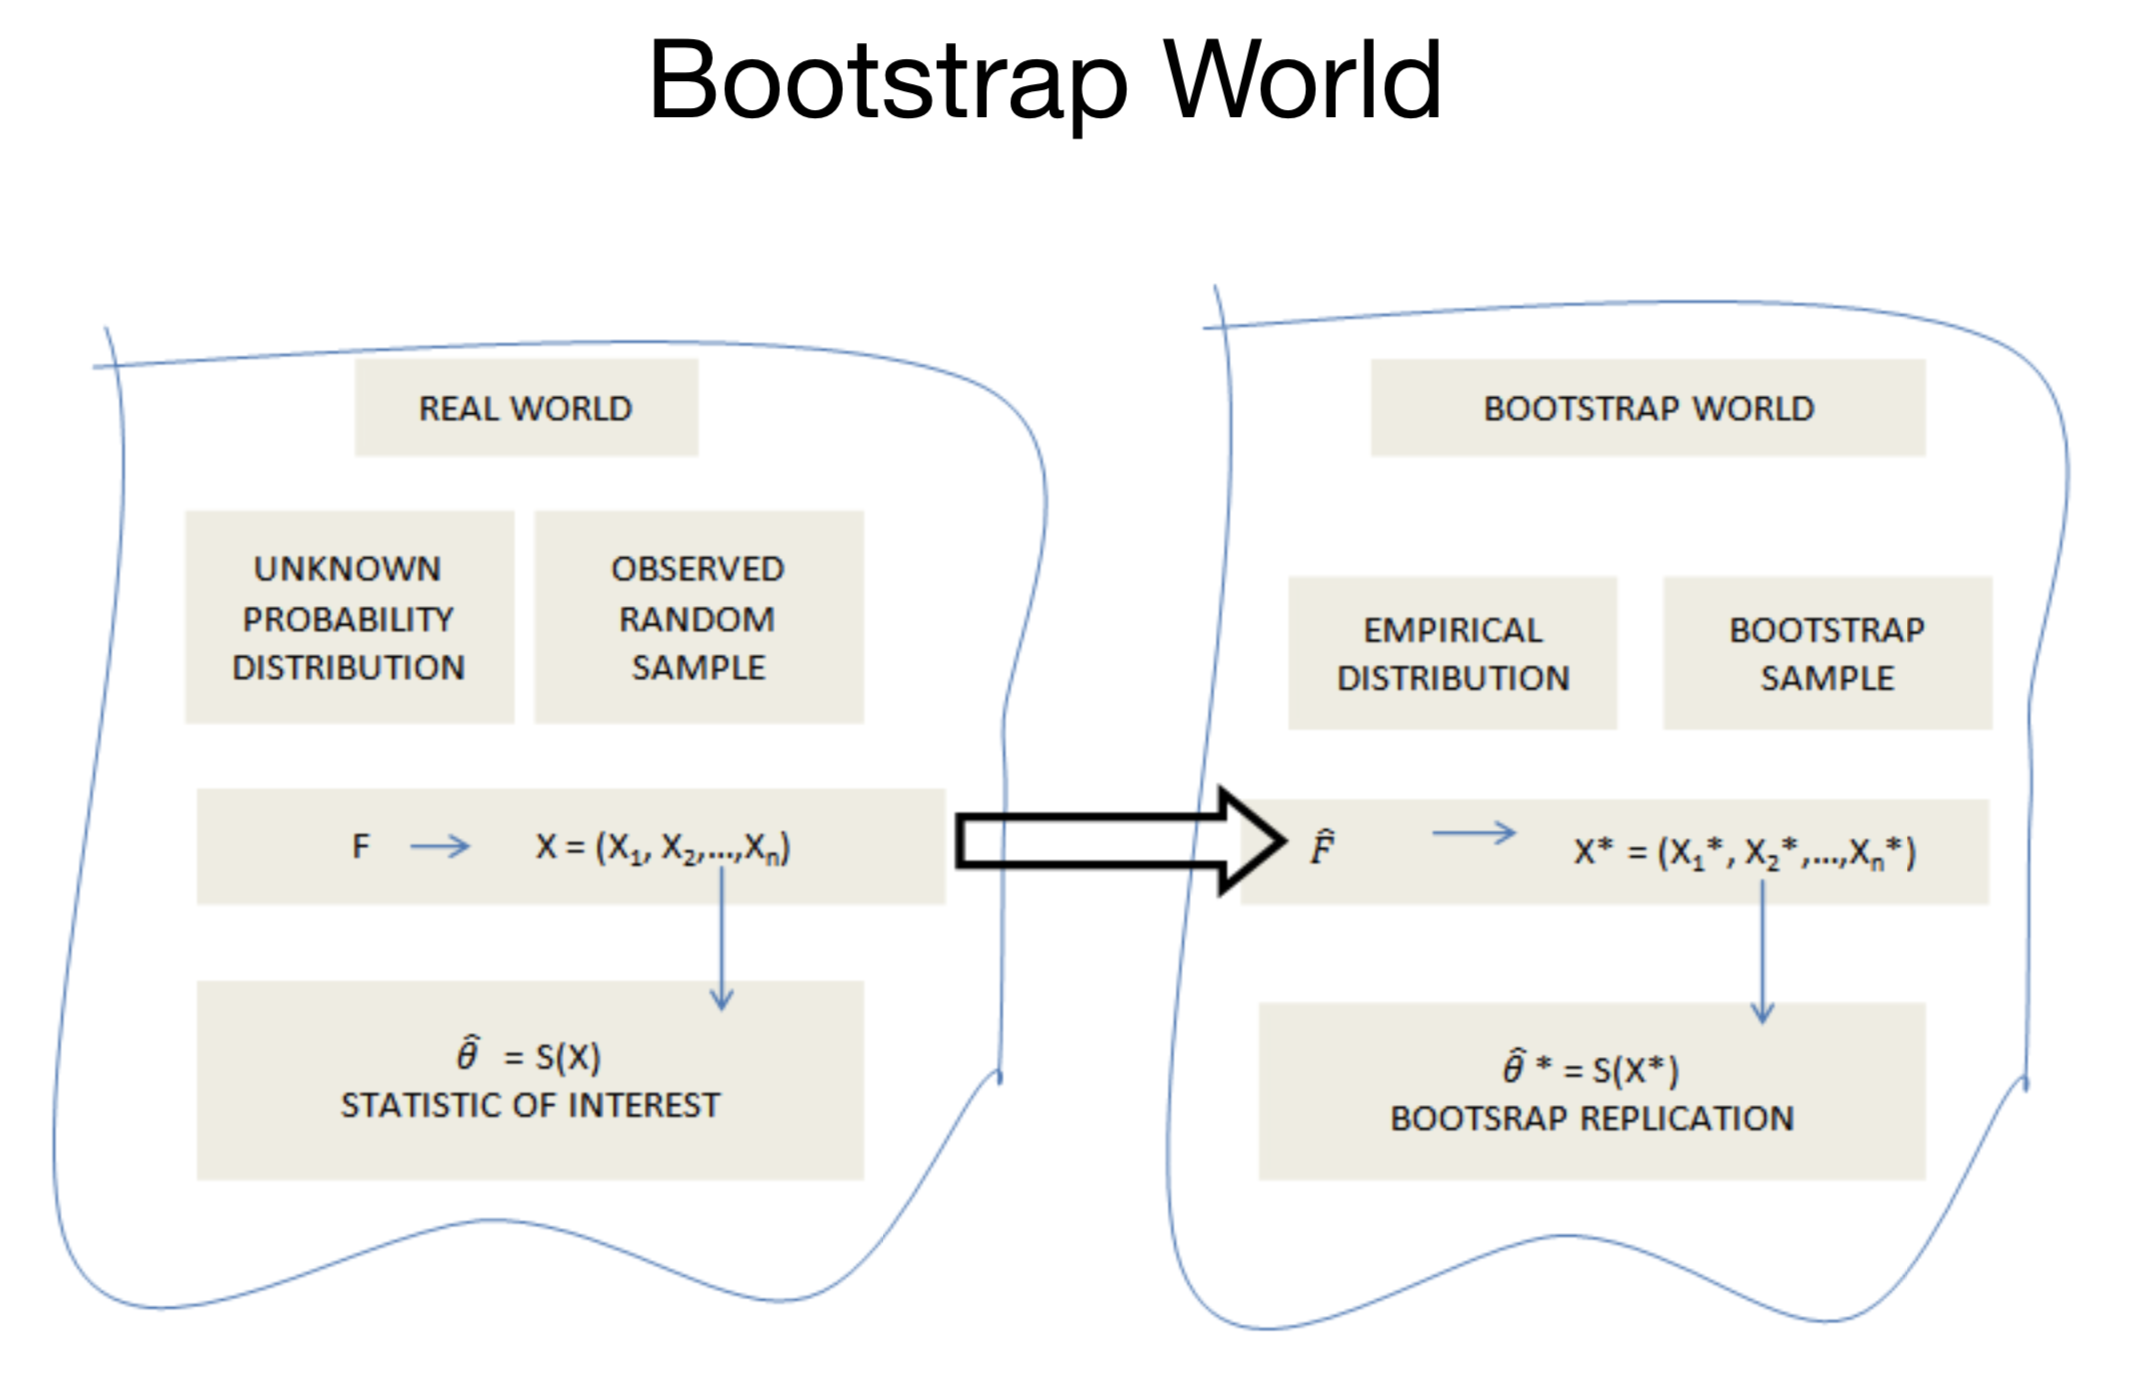
\includegraphics[width=\linewidth]{figures/bootstrap_world.png}
\end{figure}

\subsection{Sharp Null and Randomization Tests}
\begin{description}
\item[Sharp Null] $n$ units are randomized for one treatment $(X = 1)$ or another treatment $(X = 0)$. Sharp null hypothesis is
\begin{align*}
    &H_0 : y_i(1) = y_i(0) \forall i = 1, \dots , n \\
    &H_1 : y_i(1) \neq y_i(0) \text{ for some } i \in \{1, \dots, n\}
\end{align*} 
In words, the sharp \textbf{null} hypothesis says that \textit{the treatment has no effect on any individual's outcome} and the \textbf{alternative} is that \textit{the treatment has an effect for at least one individual}. 

\item[Randomization Tests]
Compute all possible ways individuals could have been randomized according to randomization protocol. For each of these ways, compute some test statistic. The p-value is the proportion of these test statistics that equal or exceed the observed test statistic. 


\section{Bayesian Statistics} \hrule height 1pt
\subsection{Basics}
Set up a probability model for quantities of interest in a problem, both  known and unknown. Then condition on the observed data, to  obtainthe posterior distribution. Two simple rules
\begin{enumerate}
    \item Always obey the laws of probability
    \item All uncertainty is to be modeled using probability
\end{enumerate}
Often controversial is the choice of the prior distribution from which we are shifting.

\textbf{Theorem: } Consider a parametric model $f(\vec{y} | \theta)$ for data $\vec{y}$, and let $\pi(\theta)$ be the prior density on the parameter $\theta$. Let $L(\theta \mid \vec{y})$ be the likelihood function. Then the posterior density of $\theta$ is proportional to the likelihood times the prior.
\begin{align*}
    \pi(\theta|\vec{y}) \propto L(\theta|\vec{y}) \pi(\theta)
\end{align*}

\subsection{Point Estimation}
\begin{description}
\item[Mean]
\begin{align*}
    \text{Prior: }& E(\theta) = \int_{-\infty}^\infty \theta \pi(\theta) \, d\theta \\ 
    \text{Posterior: }& E(\theta | \vec{y}) = \int_{-\infty}^\infty \theta \pi(\theta | \vec{y}) \, d\theta
\end{align*}
\item[Median] Value $m$ such that
\begin{align*}
    \text{Prior: }& P(\theta \leq m) \int_{-\infty}^m \pi(\theta) \, d\theta = \frac{1}{2} \\
    \text{Posterior: }& (\theta \leq m | \vec{y}) \int_{-\infty}^m \pi(\theta | \vec{y}) \, d\theta = \frac{1}{2}
\end{align*} 
\item[Mode] The prior mode is the value of $\theta$ that maximizes $\pi(\theta)$, if this value exists and is unique. The posterior mode is the value of $\theta$ that maximizes $\pi(\theta|\vec{y})$ 
\item[Squared Error Loss] $C(\theta, \hat\theta) = (\theta - \hat\theta)^2$. Expected squared error loss minimized by the \textbf{posterior mean} $E(\theta | \vec{y})$.  
\item[Absolute Error Loss] $C(\theta, \hat\theta) = |\theta - \hat\theta|$. Expected absolute error loss minimized by the \textbf{posterior median}. 
\end{description}
\end{description}

\subsection{Credible Intervals}
\begin{description}
\item[Definition] Let $0 < \alpha < 1$. A $1 - \alpha$ credible interval or posterior probabiltiy interval for a parameter $\theta$ is an interval estimator $[a(\vec{Y}), b(\vec{Y})]$ such that
\begin{align*}
    P(a(\vec{y}) \leq \theta \leq b(\vec{y}) | \vec{y}) = 1 - \alpha
\end{align*} 
Often simpler than confidence intervals, because can just look at CDF of posterior distribution. 
\end{description}

\subsection{Conjugate Priors}
\textbf{Definition} A family of priors is \textit{conjugate} for a particular model if choosing a prior in the family always results in a posterior that is in the same family.
\subsubsection{Beta-Binomial Conjugacy}
Suppose we have
\begin{align*}
    Y|p \sim \Bin(n, p)
\end{align*}
with prior 
\begin{align*}
    p \sim \Beta(a, b)
\end{align*}
Then the posterior is still Beta,
\begin{align*}
    p|(Y = y) \sim \Beta(a + y, b + n - y)
\end{align*}
\subsubsection{Poisson-Gamma Conjugacy}
Suppose we have
\begin{align*}
    Y|\lambda &\sim \Pois(\lambda t) \\
    \lambda &\sim \Gam(r_0, b_0)
\end{align*}
Then, the posterior distribution is
\begin{align*}
    \lambda|(Y = y) \sim \Gam(r_0 + y, b_0 + t)
\end{align*}
The marginal distribution of $Y$ is given by
\begin{align*}
    Y \sim \NBin\left(r_0, \frac{b_0}{b_0 + t}\right)
\end{align*}

\subsubsection{Normal-Normal Conjugacy}
The conjugate prior of mean of normal with variance know is also normal, so suppose we have
\begin{align*}
    Y|\mu &\sim \N(\mu, \sigma^2) \\
    \mu &\sim \N(\mu_0, \tau_0^2)
\end{align*}
If we define
\begin{align*}
    B = \frac{\sigma^2}{\sigma^2 + \tau_0^2}
\end{align*}
Then the posterior distribution is
\begin{align*}
    \mu|(Y = y) \sim \N((1 - B)y + B \mu_0, B \tau_0^2)
\end{align*}
and the marignal distribution of $Y$ is
\begin{align*}
    Y \sim \N(\mu_0, \sigma^2 + \tau_0^2) 
\end{align*}
The posterior mean is a weighted average of the sample mean $\bar{y}$ and the prior mean $\mu_0$. We call $B$ the \textit{shrinkage factor}.

\subsubsection{NEF Conjugacy}
Let $Y_1, \dots, Y_n$ follow the NEF
\begin{align*}
    f(y |\theta) = e^{\theta y - \psi(\theta)}h(y)
\end{align*}
Assume that $Y_1, \dots, Y_n$ are conditionally independent given $\theta$, so the likelihood functon is
\begin{align*}
    L(\theta | y) = e^{n(\theta \bar{y} - \psi(\theta))}
\end{align*}
Then a conjugate prior on $\theta$ is 
\begin{align*}
    \phi(\theta) \propto e^{r_0(\theta \mu_0 - \psi(\theta))}
\end{align*}
Furthermore, the posterior mean of the mean parameter
\begin{align*}
    \mu = E(Y_1 | \theta) = \psi'(\theta) 
\end{align*}
is a weighted average of the sample mean and the prior mean
\begin{align*}
    E(\mu|y) = (1 - B)\bar{y} + B \mu_0
\end{align*}
where
\begin{align*}
    B = \frac{r_0}{r_0 + n}
\end{align*}

\subsection{Stein's Paradox} 
\begin{description}
\item[Risk function] Given a cost function $C(\theta, \hat\theta)$, the risk function of an estimator $\hat\theta$ is its expected loss
\begin{align*}
    R(\theta) = E(C(\theta, \hat\theta) | \theta)
\end{align*} 
\item[Admissibility] An estimator $\hat\theta$ is \textit{inadmissible} if there exists another estimator whose risk fucntion is less than or equal to that of $\hat\theta$ for all possible $\theta$, with strict inequality for at least one possible value of $\theta$. An estimator is \textit{admissible} if it is not inadmissible.
\item[Inadmissibility of MLE] Let $Y_i \sim \N(\mu_i, V)$ for $i = 1, \dots, k$ be independent, where $k \geq 3$ and $\mu_i$ unknown and $V$ known. Let the estimand be $\mubold = (\mu_i, \dots, \mu_k)$ and the loss function be total squared error loss $C(\mubold, \hat\mubold) = \sum_{i = 1}^k (\mu_i - \mu)^2$. Then the MLE, which is $\vec{Y} = (Y_1, \dots, Y_k)$ is inadmissible.
\item[James-Stein estimator] Let $S = \sum_{i = 1}^k Y_i^2$. Then we have the James-Stein estimator:
\begin{align*}
    \hat\mubold_{\text{JS}} = \left(1 - \frac{(k - 2)V }{S}\right)Y_j
\end{align*}  
where $\hat\mubold_{\text{JS}}$ has strictly lower risk that $\vec{Y}, \forall \mubold \in \mathbb{R}^k$. Specifically, risk functions are
\begin{align*}
    R(\mubold, \vec{Y}) &= kV \\
    R(\mubold, \hat\mubold_{\text{JS}}) &= \left(k - (k - 2)^2 vE\left(\frac{1}{S}\right)\right)V
\end{align*}
\end{description}

\section{Canonical Examples} \hrule height 1pt
\subsubsection{MLE for Normal with Both Unknown}
By applying JFI, see that the MLE $\hat\mu=\bar{X}$ does not depend on $\sigma^2$. Plug in so the second term from JFI drops out. Set $t=\sum_{j=1}^n (x_j-\overline{x_n})^2$ (it is a constant of the data), take the derivative and find $\hat\sigma^2=\frac{t}{n}$.
\subsubsection{House Radiation Levels (Neymann-Scott)}
Suppose $\mu_i$ be the radiation level at home $i$ and that $Y_{i1},Y_{i2}\sim\N(\mu_i,\sigma^2)$, all parameters unknown, and all independent. \hide{Then we can write the likelihood function using 1) the algebra trick that $(x_1-\bar{x})^2+(x_2-\bar{x}^2)=\frac{1}{2}(x_1-x_2)^2$ (realizing that $a=x_1-\bar{x}=x_2-\bar{x}$ and then $2a^2=\frac{1}{2}(2a)^2$), and then 2) applying  JFI, so:}
\begin{align*}
L(\mu_1,\dots,\mu_n,\sigma^2	;\vec{y})&=\frac{1}{\sigma^{2n}}e^{\left(-\frac{1}{4\sigma^2}\sum_{j=1}^n(y_{j1}-y_{j2})^2-\frac{1}{\sigma^2}\sum_{j=1}^n (\bar{y_j}-\mu_j)\right)}
\end{align*}
(Solving for MLE) First stage: By inspection, we find that the MLEs are $\hat\mu_j=\overline{y_j}$. Second stage: set $\mu_j$'s above equal to the MLEs, and \textit{then} take the derivative to find $\hat\sigma_2=\frac{1}{4n}\sum_{j=1}^n (y_{j1}-y_{j2})^2$.

(Biasedness) $Y_{j1}-Y_{j2}\sim\N(0,2\sigma^2)$. $E\hat\sigma^2=\frac{2n\sigma^2}{4n}=\frac{\sigma^2}{2}$. Severe bias! Notice the MLE is off by factor by 2. Could \textbf{propose} a new estimator by multiplying by 2.

\hide{
(Why) Have to be careful. We have independent Normals, so surprising that it would be pathological. Reason: because of many $\mu_i$'s, the dimension of parameter space grows as the sample size grows (a regularity condition is not met for MLE).}
\subsubsection{German Tank Problem}
Model: Tank serial \#'s $1,2,\dots,t$, estimand $t$. Data: $n$ serial \#'s $y_1,\dots,y_n$. Simple random sample.
\begin{align*}
L(t)&=\begin{cases}
\frac{1}{\binom{t}{n}}; y_1,\dots,y_n\in\{1,\dots, t\} \\
0 \text{ otherwise}
\end{cases}	\\
&=\frac{1}{\binom{t}{n}}I(t\geq M)
\end{align*}
with $M=\max(y_1,\dots,y_n)$. By inspection, MLE is found to be $\hat t=M$. By the naive def'n of probability, we have:
\begin{align*}
P(M=m)&=\frac{\binom{m-1}{n-1}}{\binom{t}{n}} \\
EM&=\sum_{m=n}^t \frac{m\binom{m-1}{n-1}}{\binom{t}{n}}=\frac{n}{n+1}(t+1)\text{ by Feynman Stat 110 HW}
\end{align*}
We can \textit{propose} a new estimator by fixing the bias, so let $\hat t=\frac{n+1}{n}M-1$ by algebra.

We can find the MOM: $E(Y_j)=\frac{1}{t}\sum_{i=1}^t i=\frac{t+1}{2}$. So $\hat t_{\text{MOM}}=2\bar{y}-1$.

\end{multicols*}

\end{document}